% Options for packages loaded elsewhere
\PassOptionsToPackage{unicode}{hyperref}
\PassOptionsToPackage{hyphens}{url}
\PassOptionsToPackage{dvipsnames,svgnames,x11names}{xcolor}
%
\documentclass[
  number,
  preprint,
  3p,
  onecolumn]{elsarticle}

\usepackage{amsmath,amssymb}
\usepackage{iftex}
\ifPDFTeX
  \usepackage[T1]{fontenc}
  \usepackage[utf8]{inputenc}
  \usepackage{textcomp} % provide euro and other symbols
\else % if luatex or xetex
  \usepackage{unicode-math}
  \defaultfontfeatures{Scale=MatchLowercase}
  \defaultfontfeatures[\rmfamily]{Ligatures=TeX,Scale=1}
\fi
\usepackage{lmodern}
\ifPDFTeX\else  
    % xetex/luatex font selection
\fi
% Use upquote if available, for straight quotes in verbatim environments
\IfFileExists{upquote.sty}{\usepackage{upquote}}{}
\IfFileExists{microtype.sty}{% use microtype if available
  \usepackage[]{microtype}
  \UseMicrotypeSet[protrusion]{basicmath} % disable protrusion for tt fonts
}{}
\makeatletter
\@ifundefined{KOMAClassName}{% if non-KOMA class
  \IfFileExists{parskip.sty}{%
    \usepackage{parskip}
  }{% else
    \setlength{\parindent}{0pt}
    \setlength{\parskip}{6pt plus 2pt minus 1pt}}
}{% if KOMA class
  \KOMAoptions{parskip=half}}
\makeatother
\usepackage{xcolor}
\setlength{\emergencystretch}{3em} % prevent overfull lines
\setcounter{secnumdepth}{5}
% Make \paragraph and \subparagraph free-standing
\makeatletter
\ifx\paragraph\undefined\else
  \let\oldparagraph\paragraph
  \renewcommand{\paragraph}{
    \@ifstar
      \xxxParagraphStar
      \xxxParagraphNoStar
  }
  \newcommand{\xxxParagraphStar}[1]{\oldparagraph*{#1}\mbox{}}
  \newcommand{\xxxParagraphNoStar}[1]{\oldparagraph{#1}\mbox{}}
\fi
\ifx\subparagraph\undefined\else
  \let\oldsubparagraph\subparagraph
  \renewcommand{\subparagraph}{
    \@ifstar
      \xxxSubParagraphStar
      \xxxSubParagraphNoStar
  }
  \newcommand{\xxxSubParagraphStar}[1]{\oldsubparagraph*{#1}\mbox{}}
  \newcommand{\xxxSubParagraphNoStar}[1]{\oldsubparagraph{#1}\mbox{}}
\fi
\makeatother


\providecommand{\tightlist}{%
  \setlength{\itemsep}{0pt}\setlength{\parskip}{0pt}}\usepackage{longtable,booktabs,array}
\usepackage{calc} % for calculating minipage widths
% Correct order of tables after \paragraph or \subparagraph
\usepackage{etoolbox}
\makeatletter
\patchcmd\longtable{\par}{\if@noskipsec\mbox{}\fi\par}{}{}
\makeatother
% Allow footnotes in longtable head/foot
\IfFileExists{footnotehyper.sty}{\usepackage{footnotehyper}}{\usepackage{footnote}}
\makesavenoteenv{longtable}
\usepackage{graphicx}
\makeatletter
\def\maxwidth{\ifdim\Gin@nat@width>\linewidth\linewidth\else\Gin@nat@width\fi}
\def\maxheight{\ifdim\Gin@nat@height>\textheight\textheight\else\Gin@nat@height\fi}
\makeatother
% Scale images if necessary, so that they will not overflow the page
% margins by default, and it is still possible to overwrite the defaults
% using explicit options in \includegraphics[width, height, ...]{}
\setkeys{Gin}{width=\maxwidth,height=\maxheight,keepaspectratio}
% Set default figure placement to htbp
\makeatletter
\def\fps@figure{htbp}
\makeatother

\usepackage{booktabs}
\usepackage{longtable}
\usepackage{array}
\usepackage{multirow}
\usepackage{wrapfig}
\usepackage{float}
\usepackage{colortbl}
\usepackage{pdflscape}
\usepackage{tabu}
\usepackage{threeparttable}
\usepackage{threeparttablex}
\usepackage[normalem]{ulem}
\usepackage{makecell}
\usepackage{xcolor}
\usepackage{caption}
\usepackage{dcolumn}
\usepackage{typearea}
\usepackage{longtable}
\makeatletter
\@ifpackageloaded{caption}{}{\usepackage{caption}}
\AtBeginDocument{%
\ifdefined\contentsname
  \renewcommand*\contentsname{Table of contents}
\else
  \newcommand\contentsname{Table of contents}
\fi
\ifdefined\listfigurename
  \renewcommand*\listfigurename{List of Figures}
\else
  \newcommand\listfigurename{List of Figures}
\fi
\ifdefined\listtablename
  \renewcommand*\listtablename{List of Tables}
\else
  \newcommand\listtablename{List of Tables}
\fi
\ifdefined\figurename
  \renewcommand*\figurename{Figure}
\else
  \newcommand\figurename{Figure}
\fi
\ifdefined\tablename
  \renewcommand*\tablename{Table}
\else
  \newcommand\tablename{Table}
\fi
}
\@ifpackageloaded{float}{}{\usepackage{float}}
\floatstyle{ruled}
\@ifundefined{c@chapter}{\newfloat{codelisting}{h}{lop}}{\newfloat{codelisting}{h}{lop}[chapter]}
\floatname{codelisting}{Listing}
\newcommand*\listoflistings{\listof{codelisting}{List of Listings}}
\makeatother
\makeatletter
\makeatother
\makeatletter
\@ifpackageloaded{caption}{}{\usepackage{caption}}
\@ifpackageloaded{subcaption}{}{\usepackage{subcaption}}
\makeatother

\ifLuaTeX
  \usepackage{selnolig}  % disable illegal ligatures
\fi
\usepackage[]{natbib}
\bibliographystyle{elsarticle-num}
\usepackage{bookmark}

\IfFileExists{xurl.sty}{\usepackage{xurl}}{} % add URL line breaks if available
\urlstyle{same} % disable monospaced font for URLs
\hypersetup{
  pdftitle={Unveiling Adaptive Pedagogy: Reinforcement Learning Models Illuminate Teacher Decision-Making in an Online Math-Teaching Platform},
  pdfauthor={Marcos Gallo},
  pdfkeywords={Reinforcement Learning, Pedagogical Decision-Making,
Digital Education Platforms, Instructional Adaptation, Q-learning,
Actor-Critic},
  colorlinks=true,
  linkcolor={blue},
  filecolor={Maroon},
  citecolor={Blue},
  urlcolor={Blue},
  pdfcreator={LaTeX via pandoc}}


\setlength{\parindent}{6pt}
\begin{document}

\begin{frontmatter}
\title{Unveiling Adaptive Pedagogy: Reinforcement Learning Models
Illuminate Teacher Decision-Making in an Online Math-Teaching Platform}
\author[]{Marcos Gallo%
%
}



\cortext[cor1]{Corresponding author}

        
\begin{abstract}
This study introduces a new use of reinforcement learning (RL) models to
gain insight into teachers' decision-making processes on the Zearn
online math-teaching platform. Analyzing data from 3029 classrooms, our
approach treats pedagogical decision-making as a complex adaptive
system, taking into account educators' reward history and the unique
contexts of their instructional environments. Using Q-learning and
Actor-Critic models, we identify distinct patterns of teaching behavior.
Our comparison of RL models with a traditional logistic regression
baseline demonstrates the superiority of the Actor-Critic model in
capturing teacher behavior across most classrooms. Importantly, our
findings reveal a strong positive correlation between the learning rates
of state value weights and improved student achievement within the
preferred Actor-Critic model. This finding highlights educators'
adaptability in meeting their students' evolving needs in the digital
learning landscape, ultimately leading to better learning outcomes. By
demonstrating the relevance of RL models in the educational domain, our
study introduces a new approach to exploring teacher decision-making and
showcases their potential to inform the development of more effective,
adaptive teaching strategies.
\end{abstract}





\begin{keyword}
    Reinforcement Learning, Pedagogical Decision-Making, Digital
Education Platforms, Instructional Adaptation, Q-learning,
Actor-Critic \sep 
    Reinforcement Learning, Pedagogical Decision-Making, Digital
Education Platforms, Instructional Adaptation, Q-learning, Actor-Critic
\end{keyword}
\end{frontmatter}
    

\section{Introduction}\label{introduction}

Predicting repeated behavior has been a long-standing goal of the
behavioral sciences, including economics, psychology, and neuroscience
\citep{verplanken2022, venkatesh2023, hagger2023}. Reinforcement
learning (RL) algorithms have emerged as a prominent way of quantifying
these relationships, assigning a mathematical relationship between
contextual cues (states), behavior (actions), and reward
\citep{sutton2018, kaelbling1996}. These algorithms have found wide
application in neuroscience and cognitive psychology, where they are
used in data sets to model agents in specific environments
\citep{zhang2020}.

\citep{niv2022}, for example, proposed a perspective on cognitive
behavioral therapy (CBT) by framing it within reinforcement learning
(RL) theory. Highlighting the similarities between these two domains
offers a promising avenue for advancing our understanding of CBT and
refining its clinical applications. Specifically, the researchers
propose that CBT's cognitive aspect may correspond to the model-based
learning system, while its behavioral component relates to the
model-free system. There are two examples of RL applications. First,
prolonged exposure therapy (i.e., vividly recounting a traumatic
experience in a safe environment) is akin to updating the value of a
traumatic state. One novel insight from RL is that moderate prediction
errors (i.e., gradual extinction) are more effective than high
prediction errors, which can lead to new values being assigned to an
entirely different state. Second, RL theory can explain how CBT
treatments for obsessive-compulsive disorder work. Patients are asked to
imagine and write down the worst-case outcomes of not performing their
obsessions. In RL terms, this activity forces patients to create a model
of the world with low transition probabilities for worst-case scenarios,
effectively reducing the perceived probability of feared outcomes. While
this theoretical framework is compelling, future research must
substantiate these novel insights with concrete empirical evidence.

\citep{collins2020}, however, discussed the complexities of
reinforcement learning, moving beyond the traditional model-based (MB)
and model-free (MF) dichotomies. These dichotomies, while beneficial in
understanding certain aspects of human learning and decision-making,
also impose limitations by oversimplifying the diverse mechanisms at
play in RL. Such dichotomies have advanced understanding of neural and
social factors influencing behavior; however, Collins and Cockburn
pointed out the challenge of uniquely and reliably classifying behaviors
under any one controller due to the diversity and complexity of learning
mechanisms. Instead, MB and MF learning should be seen as high-level
processes emerging from coordinating various sub-computations; however,
it is important to consider independent underlying computations in MB
and MF algorithms and the potential to recombine these subcomponents
meaningfully, thereby questioning the strict separation between MB and
MF RL. From this theoretical discussion, further research is needed to
explore the complexities of reinforcement learning by refocusing on the
diverse computational components that constitute learning and
decision-making, particularly in empirical studies. The nuanced
understanding of learning processes can inform the development of more
sophisticated models to capture the diverse decision-making strategies
of teachers. This approach aligns with our goal of transcending simple
binary models to embrace the multifaceted nature of individual teacher
behavior in digital learning environments.

More pragmatically, \citep{park2019} explored the benefits of using a
personalized social robot learning companion using a model-free
Q-learning approach to improve engagement and learning outcomes among
young English language learners. Their approach employed affective
reinforcement learning to train a customized storytelling approach for
each child, optimized for their skill progression. The experiment
included 67 children between the ages of 4-6 divided into one of three
groups: personalized robot, non-personalization robot, and a no-robot
baseline. Throughout 6-8 sessions, the children participated in
storytelling activities with the robots; the personalized robot used a
model-free Q-learning approach to predict the complexity levels of the
activities to maximize a child's future engagement and learning gains.
As such, a) the reward was a combination of engagement and learning
progress (assessed through the child's use of new words and syntax
structures), b) states were the users' engagement (measured by verbal
and nonverbal cues) and affective arousal levels (measured by facial
expressions), and c) actions were the complexity level of the
activities. Results indicated that the personalized robot effectively
adapted to each child's needs, leading to better engagement and learning
outcomes than non-personalized and no-robot conditions. The positive
results suggest that a Q-learning strategy can offer tailored and
improved teaching methods. However, Park et al.~chose the model and
multiple parameters arbitrarily; therefore, future models could enhance
the robot's outcomes by, for example, defining other state spaces or
learning rates. Additionally, the generalizability of these findings to
other educational settings and populations is needed. The affective
reinforcement learning approach effectively operationalizes states,
actions, and rewards in an educational space, resulting in adaptive,
engaging learning experiences for students.

Researchers have also attempted to bridge computational neuroscience and
clinical applications. \citep{brown2021} investigated whether depression
symptoms are related to features of reinforcement learning, fitting a
state-free q-learning algorithm to participants' behavior in a reward
and loss learning task (i.e., learning a stimulus's expected monetary
gains or losses, respectively). The researchers then regressed
depression symptoms on the model-derived parameters and found that
depression symptoms may selectively disrupt specific components of the
reinforcement learning process. Notably, the Brown et al.~study bridges
computational neuroscience and clinical applications, offering a novel
way of characterizing depression, typifying patients, and opening new
avenues for personalized treatment. The study resonates with using
estimated parameters as markers of individual differences, hinting at
the potential for personalized interventions based on these models.
Likewise, our study examines the variation in estimated learning rate
parameters and their association with overall student outcomes.

In another investigation of reinforcement learning in neuroscience,
\citep{eckstein2021} reviewed the interpretability and generalizability
of reinforcement learning (RL) models in neuroscience and cognitive
science, highlighting the widely adopted assumption that estimated RL
parameters explain specific (neuro)cognitive functions and that these
explanations translate across contexts. Methodological differences among
RL studies yield a considerable variation in interpretation; for
instance, learning rates have been linked to incremental updating,
reward sensitivity, and approximate inference. Consequently,
generalizing findings across tasks, populations, and model
parameterizations is not often appropriate. Eckstein et al.~emphasized
that future research should contextualize findings within specific
experimental setups and consider alternative models that better capture
the complexities of human cognition. We take this advice to address the
degrees of freedom in our research design while contextualizing our
results accordingly.

The focus primarily on neuroscience and cognitive psychology
applications, however, presents a novel opportunity to use methods from
one set of disciplines on data traditionally used in another. In this
paper, we aim to further this integration by applying RL algorithms to
model the decision-making process of teachers in the math-teaching
platform Zearn. RL provides a system of rewards and punishments where
the agent (in this case, the teacher) learns to make optimal decisions
by maximizing the rewards and minimizing the punishments
\citep{sutton2018, kaelbling1996}. By assuming every teacher has an
objective function to balance with their potential rewards, we model the
sequential behavior of a teacher throughout a school year. For instance,
the teacher chooses which pedagogical actions to employ, such as
assigning homework, checking student progress, or reviewing content, in
anticipation of enhancing student achievement. Applying RL algorithms
allows for flexibility in learning the best strategy given certain
contextual information. We provide a model of how teachers adapt their
strategies in response to student performance and other contextual
factors. This approach offers a flexible model for our available data
and opens new avenues for understanding and enhancing human behavior in
complex, real-world settings.

\subsection{The Zearn Platform}\label{the-zearn-platform}

Zearn is a digital platform for mathematics education designed to
facilitate the teaching and learning of mathematics. About 25\% of
elementary school students and over 1 million middle school students
across the United States use Zearn \citep{zearn2024v}. Its unique blend
of hands-on teaching and immersive digital learning, paired with its
widespread adoption, provides the perfect setting for understanding how
teachers adapt their strategies to optimize student achievement.

Zearn's pedagogical approach includes interactive digital lessons using
visual aids (see Figure~\ref{fig-zearn-poster}) and real-time student
feedback. The platform's approach to mathematical concepts, such as
fractions, is particularly noteworthy. Students go through a series of
representations --- concrete, pictorial, and abstract --- each designed
to scaffold their understanding (i.e., ``breaking down'' problems, see
\citep{jumaat2014, reiser2014}) and prepare them for subsequent levels.

\begin{figure}

\centering{

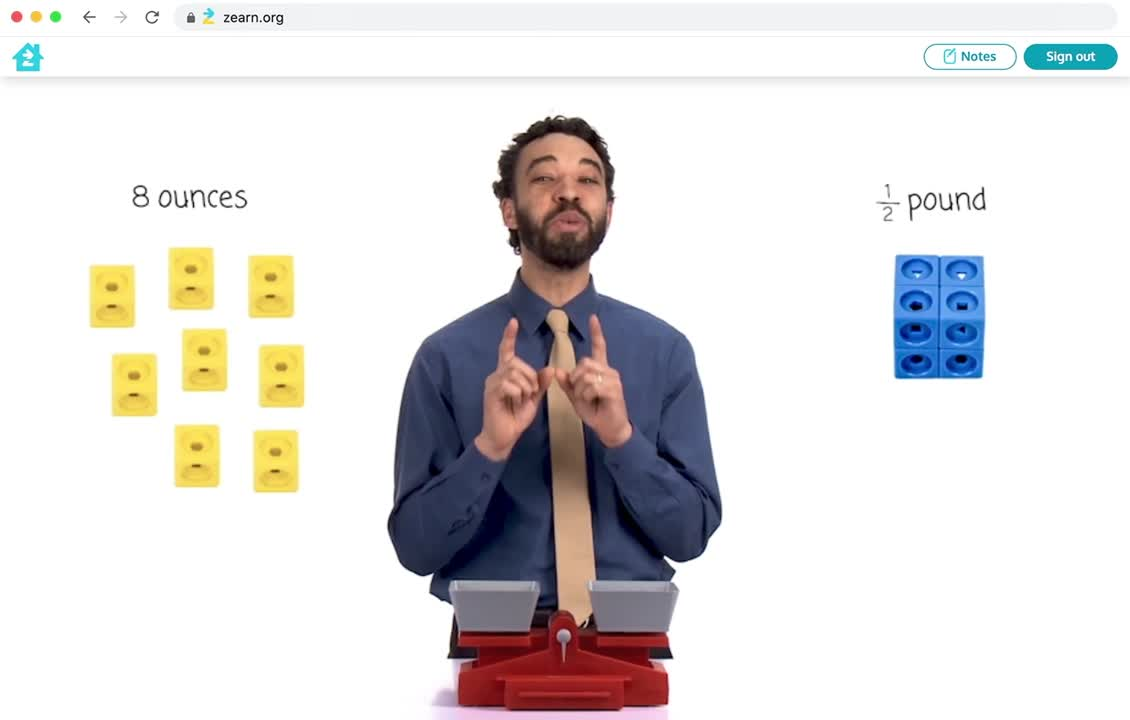
\includegraphics{images/zearn-poster.jpg}

}

\caption{\label{fig-zearn-poster}Screenshot of student lesson on Zearn.
The image is an example of teaching with visual models on the platform.}

\end{figure}%

The platform's structure provides students with a personalized learning
experience (see Appendix for a screenshot of the student portal) and
teachers with resources to track student progress and make informed
decisions (see Figure~\ref{fig-class-report} for a sample class report).
Zearn follows a rotation model of learning --- that is, a blend of
traditional face-to-face learning (i.e., small group instruction) with
online learning (i.e., self-paced online lessons). With this approach,
students can learn new grade-level content in two distinct ways:
independently, by engaging in digital lessons, and in small groups with
their teacher and peers.

\begin{figure}

\centering{

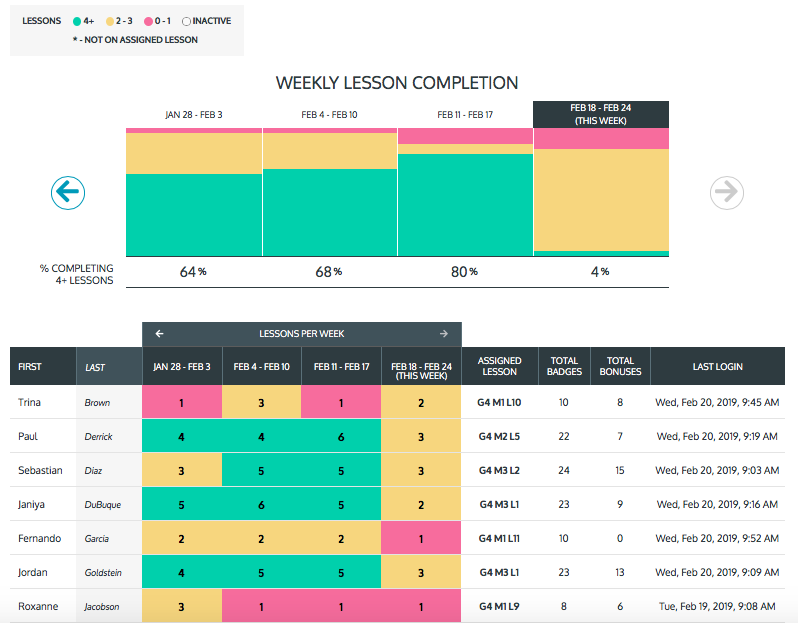
\includegraphics{images/class-report.png}

}

\caption{\label{fig-class-report}Screenshot of sample classroom report.
The image displays a summary dashboard where teachers can follow their
students' progress as indicated by the number of lessons completed.}

\end{figure}%

A key feature of Zearn is its badge system, which tracks student
progress and motivates continued learning (see
Figure~\ref{fig-badges-screen}). Students earn badges upon mastery of
specific skills, providing a tangible representation of their
achievement. This system motivates students and provides teachers with
valuable data on student performance, informing their decision-making
process \citep{knudsen2020}. Zearn also incorporates notifications,
known as Tower Alerts, sent to teachers when a student struggles with a
specific concept. This feature allows teachers to provide timely support
and address learning gaps, enhancing the platform's capacity for
personalized learning.

\begin{figure}

\centering{

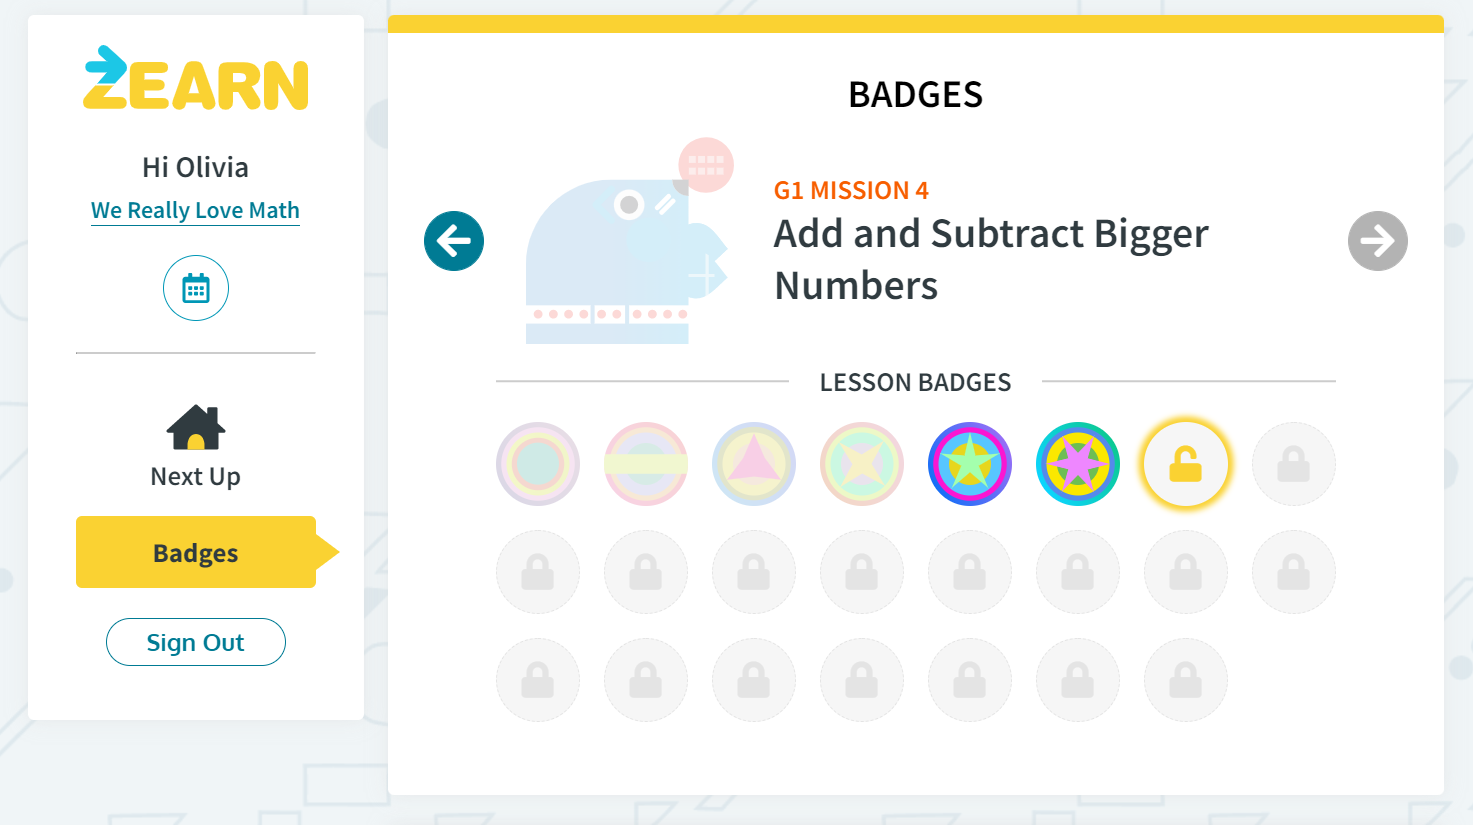
\includegraphics{images/badges.PNG}

}

\caption{\label{fig-badges-screen}Screenshot of student badges page. The
image displays a summary dashboard where students can see their total
badges earned (i.e., lessons completed) for a given mission (i.e.,
course module). Faded badges on the image signify open lessons to be
completed, unfaded badges represent earned badges, and the locked icons
correspond to future digital lessons that will open once all activities
in the current lesson are completed.}

\end{figure}%

\citep{morrison2019}, for example, evaluated the effectiveness of Zearn
Math, a digital math curriculum, in a large urban school district for
improving student outcomes. The study employed a mixed-methods approach,
combining quantitative and qualitative data from various sources,
including student achievement data, student and teacher usage data
(i.e., time spent on the platform), student and teacher surveys,
classroom observations, teacher focus groups, and administrator
interviews. The study revealed mixed results. Administrators, students,
and teachers generally viewed Zearn Math positively, citing increased
student engagement and improved instruction differentiation. However,
challenges included initial discomfort with the shift from whole class
to half-class instruction and uneven teacher preparedness, primarily due
to limited professional development opportunities. While Zearn Math
seemed to improve student engagement and higher order thinking skills,
its impact on student achievement was unclear. Achievement gains on
standardized tests were not significantly different overall, though
there were positive correlations between Zearn Math usage and
achievement gains. The program's success may be attributed to its
engaging, gamified components and alignment with the Common Core State
Standards. Additionally, it is important to provide adequate
professional development and support for teachers to effectively
implement the program. The findings of Morrison et al.~highlight the
potential and challenges of integrating digital platforms like Zearn
Math into the curriculum, which is relevant for understanding how such
tools can support teacher strategies and student engagement in
mathematics.

Another noteworthy feature is the platform's comprehensive professional
development component, which is accessible to schools with a paid
account (see Figure~\ref{fig-prof-dev} for a sample training schedule).
In this program, teachers within a school collaborate to explore each
unit or mission through word problems, fluencies, and small group
lessons. They also analyze student work and problem-solving strategies.
This professional development prioritizes (1) each mission's primary
mathematical concept, (2) visual representations to scaffold learning,
and (3) strategies to address unfinished learning from prior grades
while preparing for future learning \citep{morrison2019}.

Researchers have also examined the Zearn approach for teaching teachers
professional development knowledge. \citep{knudsen2020a} focused on the
effectiveness of the Curriculum Study Professional Development (CS PD)
program developed by Zearn to enhance elementary school teachers'
Pedagogical Content Knowledge (PCK) in teaching mathematics. The
researchers used a case study approach, examining eight teachers across
various schools and districts who had undergone the CS PD program. Data
collection methods included think-aloud interviews, classroom and CS PD
session observations, and interviews with teachers and administrators;
the researchers found that 75\% of the teachers experienced growth in
their PCK. Key strengths of the CS PD program included its relevance to
practice, encouragement of collaboration among teachers, and its
effectiveness in developing big ideas. However, challenges in responding
to students' in-the-moment problem-solving and varied teacher engagement
were noted. The findings underscore the importance of enhancing
teachers' pedagogical content knowledge, especially in mathematics. One
of the measures we developed in our study specifically captures
pedagogical content knowledge. These insights can inform the development
of similar professional development programs in the current project,
ensuring they are effectively tailored to teachers' instructional needs
and students' diverse backgrounds. Further, we are able to model teacher
behavior at the individual level.

Zearn's integrated framework provides a rich repository of data for our
analysis. The variables delineated for investigation by Zearn encompass:
(1) teacher engagement, quantified through a diverse set of actions; (2)
student achievement, denoted by variables such as lesson completion
(i.e., ``badges'' earned after each lesson is finished with full
proficiency); and (3) student struggles, monitored through variables
such as ``tower alerts'' (see Table~\ref{tbl-teacher-variables} for a
full glossary of available variables).

\subsection{Research Questions}\label{research-questions}

We propose the following research questions:

1. Characterizing Teacher Behavior: How can we best explain teachers'
action choices? How does the explanatory power of reinforcement learning
compare to simpler baseline models? Which specific reinforcement
learning model best captures the empirical data on teacher behavior?

2. Impact of Estimated RL Parameters: How do individual differences in
teachers' decision-making patterns, as inferred from the parameters of
the best-fitting reinforcement learning model, relate to heterogeneity
in student achievement gains? Can we identify specific teacher
behavioral profiles that predict better student learning outcomes?

3. Influence of Teacher and School Background: To what extent do school
contextual factors (e.g., socioeconomic status) account for variation in
teachers' instructional choices, as quantified by the parameters of the
reinforcement learning model?

\section{Theory}\label{theory}

\subsection{Reinforcement Learning to Capture Patterns in Repeated
Behavior}\label{reinforcement-learning-to-capture-patterns-in-repeated-behavior}

In RL, an agent learns to make decisions over time. Formally, an RL task
is a tuple \(\langle S,A,R,P,\gamma \rangle\), where \(S\) is a set of
states, \(A\) is a set of actions,
\(R = \mathbb{E}[R_{t+1}|S_t = s, A_t = a]\) is a reward function,
\(P= \Pr[S_{t+1} = s′ |S_t = s,A_t = a]\) is a state transition
probability, and \(\gamma \in [0,1]\) is a discount factor. We define
the agent's decisions as a probability distribution over actions,
namely, the policy \(\pi(a|s) = \Pr[A_t = a|S_t = s]\)
\citep{sutton2018}.

RL models have been used in the psychology of habit to explain learning
and reward association \citep{thorndike1931, Rescorla1972ATO}. One
common approach in human studies is to apply the ``multi-armed bandit''
task \citep{daw2006, dennison2022}. In this type of experiment,
participants are presented with multiple actions, each with an unknown
payoff. The subject's goal is to learn the best outcome through trial
and error. In the beginning, the reward-action relationships are
unknown, so the participant must explore or sample each action
\citep{sutton2018} (p.~3). This exploration-exploitation trade-off is a
central theme in RL and has the potential to provide valuable insights
into how individuals learn and make decisions over time.

In the context of education and teaching, RL has been present as early
as 1960, with Ronald Howard applying this mathematical framework to
instruction theory \citep{howard1960}. Later, in 1972, Richard Atkinson
proposed a theory of instruction that encapsulates the key components of
a Markov decision process, including states, actions, transition
probabilities, reward functions, and a time horizon
\citep{atkinson1972}. In Atkinson's framework, actions are instructional
activities (e.g., assigning problem sets) that can change a given state
(e.g., student learning level). These changes in states can yield
rewards minus the associated cost of the action. For example, a teacher
may be rewarded with an increase in the knowledge or skill of a student,
but such reward must be balanced with its associated effort (e.g., labor
cost). Atkinson and colleagues continued to test many parametrizations
of this idea, contributing significantly to the development of RL theory
in the context of education (see \citep{doroudi2019} for a full review).

In the Zearn context, we define the decision process as follows:

\begin{enumerate}
\def\labelenumi{\arabic{enumi}.}
\item
  Agents are the teachers.
\item
  Actions include the teachers' choices of specific pedagogical
  strategies.
\item
  The reward is a function of the average student performance or
  activity within a classroom.
\item
  The state is a function of other classroom variables not used in the
  reward function.
\end{enumerate}

Note that we use \(S\) in only one of our models. Further, we only
consider model-free RL algorithms, which are so called because they do
not require the agent to learn \(P\) (i.e., state transition
probabilities) to approximate expected rewards \citep{watkins1992}. In
the following sections, we describe the two models we use to capture
teacher behavior in the Zearn platform: Q-learning and Actor-Critic.

\subsection{Q-Learning Model}\label{q-learning-model}

Consider a teacher using the Zearn platform. Each week, they must decide
between two actions: assigning additional homework (action 1) or
spending more time reviewing the material in class (action 2). At first,
the teacher is uncertain about the best action to take. They start with
initial beliefs about each action's long-term value (Q-value). However,
they know that these beliefs may not be accurate and that they need to
learn from experience.

Each week, the teacher chooses an action based on the current Q-value
estimates. For example, in week 1, the teacher believes that assigning
homework (action 1) has a slightly higher Q-value than reviewing in
class (action 2). So, they assign homework and observe the outcome.

Then, the teacher receives a reward signal (e.g., the students'
performance after the homework assignment). They use this reward to
update their estimate of the Q-value for assigning homework, following
the Q-learning update rule. This rule adjusts the Q-value estimate based
on the difference between the observed reward and the previous estimate
multiplied by a learning rate parameter.

Over the following weeks, the teacher continues to make decisions and
update their estimates based on the outcomes observed. Sometimes, they
explore new actions to gather more information, even if these actions do
not seem optimal based on the current estimates. Other times, the
teacher exploits their experience by choosing the action with the
highest estimated Q-value.

As the teacher learns from experience, the Q-value estimates gradually
converge toward the true values for each action.

\begin{longtable}[]{@{}
  >{\raggedright\arraybackslash}p{(\columnwidth - 12\tabcolsep) * \real{0.0469}}
  >{\raggedright\arraybackslash}p{(\columnwidth - 12\tabcolsep) * \real{0.1562}}
  >{\raggedright\arraybackslash}p{(\columnwidth - 12\tabcolsep) * \real{0.1719}}
  >{\raggedright\arraybackslash}p{(\columnwidth - 12\tabcolsep) * \real{0.0625}}
  >{\raggedright\arraybackslash}p{(\columnwidth - 12\tabcolsep) * \real{0.0625}}
  >{\raggedright\arraybackslash}p{(\columnwidth - 12\tabcolsep) * \real{0.2422}}
  >{\raggedright\arraybackslash}p{(\columnwidth - 12\tabcolsep) * \real{0.2578}}@{}}
\caption{Example of a Q-learning algorithm for a teacher on the Zearn
platform. Each week (\(t\)), the teacher decides between action 1 and
action 2 based on the difference in Q-values (\(Q_t\)) for each action.
The teacher's choice (\(a\)) is determined by the policy
(\(\text{Pr}_t(a = 1)=1/(1+e^{-\tau Q_t})\)). After observing the reward
(\(R_t\)) associated with the chosen action, the teacher computes the
prediction error (\(\delta_t\)) using the discount factor (\(\gamma\))
and the cost (\(c\)) of the action. The Q-value is then updated using
the learning rate (\(\alpha\)) and the prediction error. As the teacher
learns from experience, the Q-value converges toward the value that
yields the highest reward. The values used here were drawn from an
actual Zearn account (\(\alpha = 0.25\), \(\tau = 10.57\),
\(\gamma = 0.46\),
\(\text{cost} = 1.38\)).}\label{tbl-qvalue-example}\tabularnewline
\toprule\noalign{}
\begin{minipage}[b]{\linewidth}\raggedright
Week
\end{minipage} & \begin{minipage}[b]{\linewidth}\raggedright
Q-value Difference
\end{minipage} & \begin{minipage}[b]{\linewidth}\raggedright
Policy
\end{minipage} & \begin{minipage}[b]{\linewidth}\raggedright
Choice
\end{minipage} & \begin{minipage}[b]{\linewidth}\raggedright
Reward
\end{minipage} & \begin{minipage}[b]{\linewidth}\raggedright
Prediction Error
\end{minipage} & \begin{minipage}[b]{\linewidth}\raggedright
Updated Q-value
\end{minipage} \\
\midrule\noalign{}
\endfirsthead
\toprule\noalign{}
\begin{minipage}[b]{\linewidth}\raggedright
Week
\end{minipage} & \begin{minipage}[b]{\linewidth}\raggedright
Q-value Difference
\end{minipage} & \begin{minipage}[b]{\linewidth}\raggedright
Policy
\end{minipage} & \begin{minipage}[b]{\linewidth}\raggedright
Choice
\end{minipage} & \begin{minipage}[b]{\linewidth}\raggedright
Reward
\end{minipage} & \begin{minipage}[b]{\linewidth}\raggedright
Prediction Error
\end{minipage} & \begin{minipage}[b]{\linewidth}\raggedright
Updated Q-value
\end{minipage} \\
\midrule\noalign{}
\endhead
\bottomrule\noalign{}
\endlastfoot
\(t\) & \(Q_t\) & \(\text{Pr}_t(a = 1)\) & \(a\) & \(R_t\) &
\(\delta_t = \gamma R_t-c-Q_t\) & \(Q_{t+1}=Q_{t}+\alpha \delta_t\) \\
1 & 1.533 & 1 & 1 & 0.052 & -2.891 & 0.815 \\
2 & 0.815 & 1 & 1 & 0.163 & -2.122 & 0.288 \\
3 & 0.288 & 0.955 & 1 & 0.047 & -1.649 & -0.121 \\
4 & -0.121 & 0.218 & 2 & 0.039 & -0.018 & -0.125 \\
5 & -0.125 & 0.210 & 2 & 0.064 & -0.030 & -0.133 \\
\ldots{} & & & & & & \\
\end{longtable}

This model frames decision-making as a result of accumulated experience
and the anticipation of future rewards. In other words, Q-learning
involves the iterative refinement of Q-value functions, which map an
agent's actions to evolving expectations of future rewards (analogous to
subjective value or utility). This methodological approach is closely
related to the classic ``multi-armed bandit'' problem, wherein the agent
faces a finite set of choices (e.g., slot machines), each linked to a
specific reward schedule, and aims to learn the action that yields the
highest returns. Learning in this model depends on adjusting
expectations to reduce the impact of prediction errors (the ``surprise
level,'' or the difference between expected and realized outcomes),
using the Bellman equation to update Q-values iteratively
\citep{rummery}.

In this study, we opt for a state-independent version of Q-learning.
That is, the Q-values do not vary with a contextual variable but are
learned for each action only. This assumption is useful in scenarios
where the state exerts minimal influence on the outcome of the action or
when the state is difficult to define or observe \citep{sutton2018}. As
such, the Q-function represents the expected return or future reward for
taking action \(a \in A = \{a_1,a_2,...\}\) following a certain policy
\(\pi = \Pr(a)\). The updating rule uses the Bellman equation as
follows:

\begin{equation}\phantomsection\label{eq-q-learn}{
Q_{t}(a) = Q_{t-1}(a) + \alpha \delta_t
}\end{equation}

where \(\alpha\) is the learning rate, which determines how much the
Q-value is updated based on \(\delta\), the reward prediction error. The
reward prediction error is the difference between the estimated Q-value
and the observed reward. This error is used to update the Q-value of the
chosen action in the direction of the observed reward, scaled by the
learning rate \(\alpha\), as follows:

\begin{equation}\phantomsection\label{eq-RPE}{
\delta_t = \gamma R_t - Q_{t-1}(a)
}\end{equation}

where:

\begin{itemize}
\item
  \(a\) is the chosen action,
\item
  \(R_t\) is the immediate reward received after taking action \(a\),
\item
  \(\gamma\) is the discount factor\footnote{Commonly, this parameter
    captures the degree to which future rewards are discounted compared
    to immediate rewards. In this example, it could also act as a
    scaling factor of net reward.},
\item
  \(Q_{t-1}(a)\) is the estimate of the Q-value for action \(a\) in the
  previous period.
\end{itemize}

In other words, \(\alpha\) is the extent to which the newly acquired
information will override the old information. A value of 0 means the
agent does not learn anything. The agent starts with an initial Q-value
(which can be arbitrary) and then updates the Q-values based on the
experiences it gathers from interactions with the environment. The
update rule is applied every time the agent takes action \(a\) and
receives a reward \(R\). The agent selects actions based on a policy
function of the Q-values. A common choice is the softmax action
selection method, which chooses actions probabilistically based on their
Q-values, as follows:

\begin{equation}\phantomsection\label{eq-softmax}{
\text{Pr}_t(a) = \frac{e^{\tau U_t(a)}}{\sum_{a'} e^{\tau U_t(a')}}
}\end{equation}

where:

\begin{itemize}
\item
  \(\Pr_t(a)\) is the probability of choosing action \(a\) at time
  \(t\),
\item
  \(U_t(a) = Q_t(a) - \text{cost}(a)\) is the utility of action \(a\) at
  time \(t\), which is the difference between the Q-value of action
  \(a\) (\(Q_t(a)\)) and the cost associated with taking that action,
\item
  \(\tau\) is a parameter known as the inverse temperature, or the
  degree of randomness in the choice behavior,\footnote{One possible
    interpretation of the inverse temperature parameter \(\tau\) is the
    agent's confidence in its Q-values, which controls the trade-off
    between exploration and exploitation. When \(\tau\) is high, the
    agent explores more because the action probabilities are more
    uniform. When \(\tau\) is low, the agent exploits more because the
    action with the highest Q-value is more likely to be chosen than the
    others. Some models may also allow for agents to start with a high
    inverse temperature to encourage exploration and then gradually
    decrease it to favor the exploitation of the learned policy.}
\item
  \(\text{cost}(a)\) is the perceived effort or inconvenience associated
  with action \(a\),
\item
  The denominator is the sum over all possible actions \(a' \in A\) of
  the exponential of their Q-values multiplied by the inverse
  temperature, and it functions as a normalizing value.
\end{itemize}

\subsubsection{Binary Actions}\label{binary-actions}

For cases in which actions are binary (i.e., only two options \(a_1\)
and \(a_2\)), we set one of the actions as an outside option with a
Q-value and cost of zero (i.e., base value \(Q(a_2)=0\) and
\(\text{cost}(a_2)=0\)). In this case, we update the difference in
Q-values, using the same Bellman equation but a modified prediction
error:

\begin{equation}\phantomsection\label{eq-state-free}{
\delta_t =
\begin{cases}
\gamma R_t - \Delta Q_{t-1} & \text{if } a_1 \text{ is chosen} \\
-\gamma R_t & \text{if } a_2 \text{ is chosen}
\end{cases}
}\end{equation}

where:

\begin{itemize}
\item
  \(\Delta Q_{t}=Q_{t}(a_1)-Q_{t}(a_2)\) is the estimate of the
  difference in Q-values for the two actions,
\item
  \(\alpha\) is the learning rate,
\item
  \(R_t\) is the immediate reward received after taking the action.
\end{itemize}

Thus, the probability of choosing a particular action is determined by
the logistic function as follows:

\[
\text{Pr}_t(a_1) = \frac{1}{1+e^{-\tau \Delta U_{t}(a)}}
\\
\text{Pr}_t(a_2) = 1 - \text{Pr}_t(a_1)
\]

where:

\begin{itemize}
\tightlist
\item
  \(\Delta U_{t}=\Delta Q_{t} - \text{cost}(a_1)\) is the estimate of
  the difference in Q-values for the two actions.
\end{itemize}

\subsection{Why Reinforcement
Learning?}\label{why-reinforcement-learning}

Reinforcement Learning (RL) presents a few advantages over models that
employ a static approach to link teacher efforts with student outcomes.
It embodies the flexibility to adapt and evolve strategies over time.
This dynamic framework reflects the continuous learning process seen in
biological systems and naturally aligns with the evolving nature of
teacher-student interactions in the classroom. Beyond our immediate
study goals, RL models hold the potential for automating instructional
decisions based on identified patterns, potentially alleviating the
workload on teachers and optimizing the educational process.

In this study, we position teachers as agents who navigate their
environment (i.e., the classroom) by taking actions based on their
observations and the feedback they receive. RL algorithms can
characterize individual profiles for teachers, providing insights into
how they adapt and respond to various states and rewards within the
educational setting. By estimating individual teacher parameters, RL
provides insights into valuable aspects for policymakers to design
targeted interventions aimed at enhancing educational outcomes.

Further, the flexibility of RL makes it an ideal tool to model how
teachers address changing classroom needs. By incorporating a wide range
of variables (i.e., states, actions, and rewards), RL models are
customizable to diverse educational contexts and objectives. Given this
flexibility in mathematically mapping the agent-environment interaction
(i.e., many models potentially satisfy our initial assumptions), our
first step is a competition of models, selecting a set of models
applicable to our setting, fitting them to the data, and comparing their
performances.

\section{Results}\label{results}

\subsection{Selecting a model
specification}\label{selecting-a-model-specification}

To analyze Zearn data spanning an entire academic year, we first
establish a framework for actions and rewards. In this framework,
teacher activities drive the educational process, student achievements
result from these efforts, and the constantly changing educational
environment represents the states. Instead of relying solely on one
analytical approach, our strategy involves a large set of candidate
models, progressively escalating in complexity, as shown in
Table~\ref{tbl-methods}. Our overarching goal was to strengthen the
reliability of our findings and offer a detailed understanding of the
underlying behavioral patterns.

\subsection{Dimensionality Reduction}\label{dimensionality-reduction}

We first conducted a dimensionality reduction with Non-negative Matrix
Factorization (NMF) and four components (see
\textbf{?@fig-nmf-pca-comparison} for a comparison of different methods
by balancing reconstruction accuracy, i.e., R-squared, with clustering
clarity, i.e., Silhouette Scores). While our dataset offers many
potential action and reward variables, the direct use of these variables
presents significant challenges:

\begin{enumerate}
\def\labelenumi{\arabic{enumi}.}
\tightlist
\item
  \textbf{Complexity}: The sheer number of available variables
  complicates the identification of meaningful patterns and
  relationships.
\item
  \textbf{Dimensionality}: The high-dimensional nature of the data risks
  diluting important signals due to the ``curse of
  dimensionality.''\footnote{Richard Bellman coined this phrase to
    describe the challenge of optimizing a control process by searching
    over a discrete multidimensional grid, where the number of grid
    points increases exponentially with the number of dimensions. He
    wrote: ``In view of all that we have said in the foregoing sections,
    the many obstacles we appear to have surmounted, what casts the pall
    over our victory celebration? It is the curse of dimensionality, a
    malediction that has plagued the scientist from the earliest days''
    \citep{bellman2015adaptive}.}
\item
  \textbf{Interpretability}: Directly interpreting the impact of
  specific actions or behaviors on outcomes can be obscured by the
  intertwined nature of the data.
\end{enumerate}

By reducing the data to a manageable number of components, we can more
readily identify underlying patterns of behavior and interaction. To
achieve this, we applied Nonnegative Matrix Factorization (NMF) and used
the results to define action, reward, and state variables rather than
using individual metrics. One desirable feature of NMF is that it
produces sparse components, providing a distilled representation of the
data, where each one reflects a combination of behaviors or activities
with a potential thematic linkage. Given that our chosen RL models
require discreet action variables, we choose to split teacher actions
into binary variables, following a median split. In our case, a median
split is equivalent to giving a value of 1 to any positive value.

\begin{verbatim}
702
\end{verbatim}

\paragraph{Interpreting Components}\label{interpreting-components}

After analyzing the NMF data, we identified four significant components
for teachers and students. Figure~\ref{fig-nmf-heatmap} displays these
components as heatmaps, offering insight into the underlying behavioral
structures. Given the loadings, we interpret the components as follows:

\subparagraph{Teachers Components}\label{teachers-components}

\textbf{Component 1 (Assessments)}: This component has substantial
weights on supplemental assessment materials, such as ``Optional Problem
Sets Download,'' ``Optional Homework Download,'' and ``Student Notes and
Exit Tickets Download,'' indicating a proactive approach to evaluating
and supporting student learning progress. It could also reflect a
proactive approach to monitoring student understanding and providing
feedback.

\textbf{Component 2 (Pedagogical Knowledge)}: The high weights on
``Guided Practice Completed,'' ``Tower Completed,'' ``Tower Stage
Failed,'' and ``Fluency Completed'' suggest that this component reflects
when teachers are engaged in acquiring subject-matter-specific pedagogy,
learning to scaffold and explain concepts in various ways.

\textbf{Component 3 (Group Instruction)}: This component, with prominent
weights on ``Small Group Lesson Download,'' ``Whole Group Word Problems
Download,'' and ``Whole Group Fluency Download,'' suggests a pedagogical
approach focused on fostering interactive and comprehensive classroom
instruction. It implies engagement in activities that promote group
learning dynamics and collective problem-solving skills.

\textbf{Component 4 (Curriculum Planning)}: The dominance of ``Mission
Overview Download'' and ``Grade Level Overview Download'' in this
component suggests that teachers are highly involved in strategic
planning and curriculum mapping. It involves organizing the curriculum
content and structuring lesson plans to align with grade-level
objectives and mission overviews.

\subparagraph{Student Components}\label{student-components}

\textbf{Component 1 (Badges)}: This component emphasizes ``On-grade
Badges'' and ``Badges,'' indicating that it measures students' overall
engagement and advancement through the curriculum.

\textbf{Component 2 (Struggles)}: This component, which heavily weights
``Boosts'' and ``Tower Alerts,'' seems to capture the frequency of
occasions when students require additional scaffolding and assistance.

\textbf{Component 3 (Number of Students)}: This component mainly
consists of ``Active Students,'' which provides insight into what
proportion of students regularly log in to complete Digital Lessons.

\textbf{Component 4 (Activity)}: Dominated by ``Student Minutes'' and
``Student Logins,'' this component highlights the amount of time
students invest in and the frequency of their interactions with Zearn.

\begin{figure}

\begin{minipage}{\linewidth}

\centering{

\includegraphics{zearn_files/figure-pdf/fig-nmf-heatmap-1.pdf}

}

\subcaption{\label{fig-nmf-heatmap-1}Teacher Data. Component 1
(Assessments) focuses on using supplemental materials for student
evaluation; Component 2 (Pedagogical Knowledge) emphasizes developing
subject-specific teaching strategies; Component 3 (Group Instruction)
centers on collaborative and whole-class teaching methods; Component 4
(Curriculum Planning) highlights planning and lesson preparation.}

\end{minipage}%
\newline
\begin{minipage}{\linewidth}

\centering{

\includegraphics{zearn_files/figure-pdf/fig-nmf-heatmap-2.pdf}

}

\subcaption{\label{fig-nmf-heatmap-2}Student Data. Component 1 (Badges)
measures curriculum engagement and progression; Component 2 (Struggles)
indicates the need for additional academic support; Component 3 (Number
of Students) tracks student participation within the platform; Component
4 (Activity) reflects the overall time spent and frequency of platform
usage.}

\end{minipage}%

\caption{\label{fig-nmf-heatmap}Heatmap of Non-negative Matrix
Factorization (NMF) components for teacher and student data. The rows
represent the original variables, and the columns correspond to the
components. The color gradient indicates the relative importance of each
variable within a component based on the proportion of the component's
total weight attributed to that variable. These proportions were
calculated by normalizing each variable weight within a component so
that they all sum to 1. To provide context, the heatmaps label examples
of low, moderate, and high proportion values.}

\end{figure}%

\subsubsection{Feature Selection}\label{feature-selection}

In order to pre-select the most appropriate action and reward variables,
we \ldots{} \citep{lau2005}. This approach acted as a filter to capture
the action-reward (or action-reward-state) configurations displaying
characteristics reminiscent of reinforcement learning (RL). We applied
four criteria: a) the influence of consistent rewards on the propensity
of actions being repeated, b) the immediate impact of states on action
selection, c) the strategic role of actions in navigating towards
desirable states, and d) the identification of action auto-correlation
as an indicator of incremental learning processes.

Herein, the interaction between lagged rewards and actions aimed to
capture the reinforcement aspect (a), where prior rewards enhance the
likelihood of repeating specific actions. Including current state
variables addressed (b) and examining how present educational contexts
inform action choices. The interaction between current states and lagged
actions encapsulated (c) that actions are deliberately chosen to
navigate towards or sustain preferable educational states. Lastly,
considering lagged rewards alone, we sought to elucidate (d) the
phenomenon where past successes influence future endeavors, indicative
of a learning trajectory.

We first explore reinforcement learning (RL)-like characteristics within
the teacher and classroom usage data. We aimed to uncover patterns
indicative of RL, where actors (teachers) select actions (teaching
strategies) that historically yield higher rewards (improved student
outcomes) and use states (classroom contexts) as signals for action
selection. Further, we sought to understand how actions contribute to
achieving or maintaining desired states and the extent to which actions
exhibit auto-correlation due to incremental learning processes.

In order to capture the temporal dynamics of actions influenced by
lagged rewards and states, we employed panel logistic regression models
across different combinations of variables and lags. We incorporate
lagged variables (ranging from one to six weeks) into the models using
the Dynamic Analysis approach proposed to account for temporal
autocorrelation and potential delayed effects. We applied reward and
state structures extracted from classroom data via non-negative matrix
factorization (NMF) with the Frobenius Non-negative Double Singular
Value Decomposition (NNDSVD) and actions derived similarly from teacher
data. We evaluate these models using the Bayesian Information Criterion
(BIC) for model complexity and fit and the Area Under the Receiver
Operating Characteristic curve (AUC) for predictive accuracy.

More specifically, we select one teacher component as the action and one
student component as the reward. When constructing state-based models,
we incorporate an additional student component as the state variable.
This choice yields 16 models (4 possible actions and 4 possible
rewards).

\subsection{Model Performance and Behavioral
Signatures}\label{model-performance-and-behavioral-signatures}

Drawing on the resulting metrics, we strategically narrowed our focus to
the action-reward-state configurations that most closely align with
Reinforcement Learning (RL) principles. \textbf{?@fig-RL-exploration}
delineates the top models based on their high fixed-effects Area Under
the Curve (AUC) and mean teacher-specific AUC, as well as their Fixed
Effects Bayesian Information Criterion (BIC) and higher mean
teacher-specific log-likelihood. Panels A and B of the figure show the
state-free and state-dependent models, respectively. Each point on the
plot represents a different model, identified by its BIC and average
teacher-specific AUC. The actions ``Pedagogical Knowledge'' and ``Group
Instruction'' stand out for both models. However, the choice of
associated rewards and states is unclear, suggesting the need to fit RL
models using all configurations featuring these two actions.

\subsubsection{Estimating RL Models}\label{estimating-rl-models}

The next step is to identify and evaluate reinforcement learning (RL)
models that best represent the teaching strategies derived from our
data. The performance of each model is quantified by computing the
Bayesian Information Criterion (BIC). Our computational analysis
identified a distinct group of models that excelled in their low BIC
scores. Table~\ref{tbl-top-CBM} provides a breakdown of scores for
different combinations of rewards and states under this action, offering
insight into the comparative performance of various model setups.
Notably, all top-performing models featured ``Pedagogical Knowledge'' as
their primary action. Models with ``Badges'' and ``Activity'' as their
rewards outperform others, as do state-free models, likely due to their
higher simplicity.

\begin{longtable}{l|lrrrr}

\caption{\label{tbl-top-CBM}Model comparison based on log-likelihood.
The table presents log-likelihood values for different models across
various action-reward combinations. Less negative values indicate better
fit. All models are compared against a baseline intercept-only
regression model. The cost-free Q-learning models do not include a cost
parameter and assume the starting q-value to be zero. Across all models,
the `Pedagogical Knowledge' action shows the best fit overall. Note that
these estimates are not hierarchical; they represent the individual
estimates of each teacher.}

\tabularnewline

\caption*{
{\large Model Comparison - Log Likelihood}
} \\ 
\toprule
\multicolumn{1}{l}{Action} & Reward & Q-learning & Q-learning (cost-free) & Lau \& Glimcher & Baseline \\ 
\midrule\addlinespace[2.5pt]
Assessments & Badges & $-24,208.42$ & $-27,425.17$ & $-24,831.02$ & $-27,176.43$ \\ 
 & Struggles & $-24,283.40$ & $-27,709.75$ & $-24,833.22$ & $-27,176.43$ \\ 
 & No. Students & $-24,252.29$ & $-27,108.38$ & $-24,907.33$ & $-27,176.43$ \\ 
 & Activity & $-24,220.46$ & $-27,373.89$ & $-24,827.77$ & $-27,176.43$ \\ 
\midrule\addlinespace[2.5pt]
Pedagogical Knowledge & Badges & $-20,900.34$ & $-25,291.43$ & $-21,189.95$ & $-23,605.37$ \\ 
 & Struggles & $-20,900.96$ & $-25,531.27$ & $-21,193.80$ & $-23,605.37$ \\ 
 & No. Students & $-20,906.79$ & $-25,046.88$ & $-21,253.18$ & $-23,605.37$ \\ 
 & Activity & $-20,910.36$ & $-25,213.89$ & $-21,175.05$ & $-23,605.37$ \\ 
\midrule\addlinespace[2.5pt]
Group Instruction & Badges & $-23,788.51$ & $-27,688.01$ & $-24,540.78$ & $-27,181.44$ \\ 
 & Struggles & $-23,835.75$ & $-27,935.43$ & $-24,552.94$ & $-27,181.44$ \\ 
 & No. Students & $-23,800.23$ & $-27,530.45$ & $-24,618.32$ & $-27,181.44$ \\ 
 & Activity & $-23,771.94$ & $-27,591.98$ & $-24,537.39$ & $-27,181.44$ \\ 
\midrule\addlinespace[2.5pt]
Curriculum Planning & Badges & $-24,661.42$ & $-28,315.00$ & $-24,900.79$ & $-26,967.87$ \\ 
 & Struggles & $-24,669.08$ & $-28,564.54$ & $-24,903.75$ & $-26,967.87$ \\ 
 & No. Students & $-24,687.01$ & $-28,262.99$ & $-24,980.06$ & $-26,967.87$ \\ 
 & Activity & $-24,687.32$ & $-28,256.58$ & $-24,900.18$ & $-26,967.87$ \\ 
\bottomrule

\end{longtable}

\subsubsection{Hierarchical Bayesian Inference (HBI) Results and Model
Comparison}\label{hierarchical-bayesian-inference-hbi-results-and-model-comparison}

To further refine our selection, we employ Hierarchical Bayesian
Inference (HBI) to perform a more detailed comparison of the selected
models. This statistical approach allows us to compare models not just
by their individual fits but also by their ability to explain data
across different subjects. In interpreting the results from HBI, we
observed the differential performances of Q-learning (QL) and
Actor-Critic (AC) models. \textbf{?@tbl-CBM-HBI} provides quantifiable
insights into each model's fit (BIC) and predictive power (AUC, the area
under the receiver operating characteristic curve) across teachers.
Generally, Q-learning models fit the data better than Actor-Critic
models (i.e., lower BIC scores), and AC models outperform in terms of
predictive power (higher AUC scores).

\begin{longtable}{ccc}

\caption{\label{tbl-model-summary}Summary of model fits for Pedagogical
Knowledge as actions and Badges as rewards. Each of the models
(N\textsubscript{par} = number of parameters) was fitted to participants
data using Matlab's cbm toolbox. Using individual model-fitting, we
computed the mean AIC (lower values indicate better model fit).}

\tabularnewline

\toprule
Model & N\textasciitilde{}par\textasciitilde{} & AIC \\ 
\midrule\addlinespace[2.5pt]
Q-learning & 5 & $32.8$ \\ 
Q-learning (cost-free) & 3 & $33.6$ \\ 
Lau \& Glimcher & 5 & $33.1$ \\ 
Baseline & 1 & $27.8$ \\ 
\bottomrule

\end{longtable}

\subsection{Posterior Predictive
Checks}\label{posterior-predictive-checks}

\begin{verbatim}
[[1]]
\end{verbatim}

\begin{verbatim}

[[2]]
\end{verbatim}

\begin{figure}

\centering{

\includegraphics{zearn_files/figure-pdf/fig-reward-seeking-1.pdf}

}

\caption{\label{fig-reward-seeking-1}Reward-seeking behavior. The graphs
compare three models (Q-learning, Lau \& Glimcher, and Baseline) in
their ability to capture teachers' reward-seeking behavior. The x-axis
represents the percentile of the difference in Q-values between action
and inaction. The y-axis shows the proportion of times teachers chose to
act. Black points represent mean proportions observed across teachers,
with error bars depicting the standard error of these means. The dashed
black line represents the smoothed trend of observed teacher behavior.
Colored lines and shaded areas show model predictions with 95\%
confidence intervals.}

\end{figure}%

\begin{figure}

\centering{

\includegraphics{zearn_files/figure-pdf/fig-reward-seeking-2.pdf}

}

\caption{\label{fig-reward-seeking-2}Reward-seeking behavior. The graphs
compare three models (Q-learning, Lau \& Glimcher, and Baseline) in
their ability to capture teachers' reward-seeking behavior. The x-axis
represents the percentile of the difference in Q-values between action
and inaction. The y-axis shows the proportion of times teachers chose to
act. Black points represent mean proportions observed across teachers,
with error bars depicting the standard error of these means. The dashed
black line represents the smoothed trend of observed teacher behavior.
Colored lines and shaded areas show model predictions with 95\%
confidence intervals.}

\end{figure}%

\begin{verbatim}
[[1]]
\end{verbatim}

\begin{verbatim}

[[2]]
\end{verbatim}

\begin{figure}

\centering{

\includegraphics{zearn_files/figure-pdf/fig-uncertainty-aversion-1.pdf}

}

\caption{\label{fig-uncertainty-aversion-1}Uncertainty aversion. The
graphs compare three models (Q-learning, Lau \& Glimcher, and Baseline)
in their ability to capture teachers' uncertainty-related behavior. The
x-axis represents the percentile of the difference in expected value
(EV) between uncertain and certain options, calculated from the
cumulative means and standard deviations of rewards associated with each
action. The y-axis shows the proportion of times teachers chose the
uncertain option. Black points represent mean proportions observed
across teachers, with error bars depicting the standard error of these
means. The dashed black line represents the smoothed trend of observed
teacher behavior. Colored lines and shaded areas show model predictions
with 95\% confidence intervals. The horizontal dashed line at 50\%
represents indifference between certain and uncertain options.}

\end{figure}%

\begin{figure}

\centering{

\includegraphics{zearn_files/figure-pdf/fig-uncertainty-aversion-2.pdf}

}

\caption{\label{fig-uncertainty-aversion-2}Uncertainty aversion. The
graphs compare three models (Q-learning, Lau \& Glimcher, and Baseline)
in their ability to capture teachers' uncertainty-related behavior. The
x-axis represents the percentile of the difference in expected value
(EV) between uncertain and certain options, calculated from the
cumulative means and standard deviations of rewards associated with each
action. The y-axis shows the proportion of times teachers chose the
uncertain option. Black points represent mean proportions observed
across teachers, with error bars depicting the standard error of these
means. The dashed black line represents the smoothed trend of observed
teacher behavior. Colored lines and shaded areas show model predictions
with 95\% confidence intervals. The horizontal dashed line at 50\%
represents indifference between certain and uncertain options.}

\end{figure}%

\begin{verbatim}
[[1]]
\end{verbatim}

\begin{verbatim}

[[2]]
\end{verbatim}

\begin{figure}

\centering{

\includegraphics{zearn_files/figure-pdf/fig-prediction-errors-1.pdf}

}

\caption{\label{fig-prediction-errors-1}Learning curves. The plots show
the mean reward prediction errors across teachers over time. The x-axis
represents biweekly periods throughout the school year. The solid line
represents mean values and the shaded area represents the standard error
of the mean. A dashed horizontal line at y=0 serves as a reference for
zero prediction error. The curve illustrates a general trend of
increasing prediction accuracy (decreasing absolute prediction error)
until March.}

\end{figure}%

\begin{figure}

\centering{

\includegraphics{zearn_files/figure-pdf/fig-prediction-errors-2.pdf}

}

\caption{\label{fig-prediction-errors-2}Learning curves. The plots show
the mean reward prediction errors across teachers over time. The x-axis
represents biweekly periods throughout the school year. The solid line
represents mean values and the shaded area represents the standard error
of the mean. A dashed horizontal line at y=0 serves as a reference for
zero prediction error. The curve illustrates a general trend of
increasing prediction accuracy (decreasing absolute prediction error)
until March.}

\end{figure}%

\begin{verbatim}
$`2`
\end{verbatim}

\begin{verbatim}

$`14`
\end{verbatim}

\begin{figure}

\centering{

\includegraphics{zearn_files/figure-pdf/fig-q-value-reward-diff-1.pdf}

}

\caption{\label{fig-q-value-reward-diff-1}Q-value and reward differences
over time. The x-axis represents biweekly periods throughout the school
year. The y-axis shows the difference in Q-values or mean rewards
between action and inaction. Shaded areas represent the standard error
of the mean.}

\end{figure}%

\begin{figure}

\centering{

\includegraphics{zearn_files/figure-pdf/fig-q-value-reward-diff-2.pdf}

}

\caption{\label{fig-q-value-reward-diff-2}Q-value and reward differences
over time. The x-axis represents biweekly periods throughout the school
year. The y-axis shows the difference in Q-values or mean rewards
between action and inaction. Shaded areas represent the standard error
of the mean.}

\end{figure}%

\begin{verbatim}
$`2`
\end{verbatim}

\begin{verbatim}

$`14`
\end{verbatim}

\begin{figure}

\centering{

\includegraphics{zearn_files/figure-pdf/fig-action-percentages-1.pdf}

}

\caption{\label{fig-action-percentages-1}Observed teacher behavior and
model predictions over the academic year. The graph shows the percentage
of times teachers chose to engage in Pedagogical Content activities. The
x-axis represents biweekly periods throughout the school year. The black
dashed line represents observed teacher behavior, while colored lines
represent predictions from different models. Shaded areas represent the
95\% confidence intervals for each model's predictions.}

\end{figure}%

\begin{figure}

\centering{

\includegraphics{zearn_files/figure-pdf/fig-action-percentages-2.pdf}

}

\caption{\label{fig-action-percentages-2}Observed teacher behavior and
model predictions over the academic year. The graph shows the percentage
of times teachers chose to engage in Pedagogical Content activities. The
x-axis represents biweekly periods throughout the school year. The black
dashed line represents observed teacher behavior, while colored lines
represent predictions from different models. Shaded areas represent the
95\% confidence intervals for each model's predictions.}

\end{figure}%

\subsubsection{Top Model Selection}\label{top-model-selection}

\textbf{?@tbl-CBM-second} also shows that Q-learning consistently
outperforms logistic regression and actor-critic models in BIC scores.
As such, we further analyze the fit from the top models from this table
to the entire dataset. That is, we compare both Q-learning models and
the top actor-critic model with their corresponding logistic regression.
The histogram of teacher-specific log-likelihoods in
Figure~\ref{fig-loglik-histogram} reveals that the Q-learning model with
``Struggles'' as the reward has the lowest BIC scores.

\subsection{Heterogeneity and
Optimality}\label{heterogeneity-and-optimality}

The spread of BIC scores in Figure~\ref{fig-loglik-histogram} also
implies a diversity in model fit, which warrants further investigation
into heterogeneity. We analyzed teacher-specific parameters to capture
these individual differences. \textbf{?@fig-params-histogram} provides a
set of visualizations depicting relationships between teacher-specific
parameters and various contextual factors. We observed differences in
the cost parameter across poverty levels, with high-poverty schools
showing lower cost estimates (a). The learning rate parameter (alpha)
also varied across poverty levels (b), with high-poverty schools
exhibiting lower learning rates. The number of weeks a teacher used the
platform showed a small negative correlation with the estimated cost (r
= -0.11, p \textless{} .001) (d), while it positively correlated with
the inverse temperature parameter (tau) (r = 0.14, p = 1.5e-09) (e).
When examining the relationship between the learning rate, inverse
temperature, and student outcomes (c, f), we found a positive
correlation between inverse temperature and both average badges (r =
0.17, p \textless{} .001) and average tower alerts (r = 0.1, p
\textless{} .001). However, the learning rate did not significantly
correlate with average badges earned (r = 0.03, p = 0.23) or average
tower alerts (r = 0.0, p = .85).

\begin{table}

\caption{\label{tbl-optimality}Impact of Q-learning Model Parameters on
Average Weekly Badges Earned per Student. Three linear regression models
examine the correlations between a teacher's reinforcement learning (RL)
parameters and student engagement, measured by average weekly badges
earned per student. Model 1 includes only RL parameters. Model 2 adds
controls for AIC, number of weeks, total students, and number of
classes. Model 3 further incorporates controls for grade level, poverty
level, charter school status, and whether the school has a paid Zearn
account. Coefficients and standard errors (in parentheses) are provided
for each parameter.}

\centering{

[!htbp] \centering 
  \caption{} 
  \label{} 
\begin{tabular}{@{\extracolsep{5pt}}lD{.}{.}{-3} D{.}{.}{-3} D{.}{.}{-3} } 
\\[-1.8ex]\hline 
\hline \\[-1.8ex] 
 & \multicolumn{3}{c}{\textit{Dependent variable:}} \\ 
\cline{2-4} 
\\[-1.8ex] & \multicolumn{3}{c}{Badges} \\ 
\\[-1.8ex] & \multicolumn{1}{c}{(1)} & \multicolumn{1}{c}{(2)} & \multicolumn{1}{c}{(3)}\\ 
\hline \\[-1.8ex] 
 $\alpha$ & 0.050^{**} & 0.074^{***} & 0.061^{***} \\ 
  & (0.015) & (0.015) & (0.015) \\ 
  & & & \\ 
 $\gamma$ & -0.088^{***} & -0.081^{***} & -0.083^{***} \\ 
  & (0.018) & (0.017) & (0.017) \\ 
  & & & \\ 
 $\tau$ & 0.046^{**} & 0.054^{***} & 0.046^{**} \\ 
  & (0.015) & (0.015) & (0.015) \\ 
  & & & \\ 
 Cost & 0.014 & 0.058^{**} & 0.047^{*} \\ 
  & (0.016) & (0.021) & (0.021) \\ 
  & & & \\ 
 Starting Q-value & -0.111^{***} & -0.059^{**} & -0.057^{**} \\ 
  & (0.017) & (0.018) & (0.018) \\ 
  & & & \\ 
 No. of Weeks &  & 0.012^{***} & 0.010^{***} \\ 
  &  & (0.003) & (0.003) \\ 
  & & & \\ 
 No. of Students &  & 0.001 & 0.001 \\ 
  &  & (0.002) & (0.002) \\ 
  & & & \\ 
 No. of Classes &  & -0.124^{***} & -0.124^{***} \\ 
  &  & (0.013) & (0.016) \\ 
  & & & \\ 
 Charter School &  &  & -0.096 \\ 
  &  &  & (0.053) \\ 
  & & & \\ 
 Paid Zearn Account &  &  & 0.218^{***} \\ 
  &  &  & (0.039) \\ 
  & & & \\ 
 Constant & 1.558^{***} & 1.190^{***} & 1.627^{***} \\ 
  & (0.013) & (0.079) & (0.175) \\ 
  & & & \\ 
\hline \\[-1.8ex] 
Control for AIC &  & Yes & Yes \\ 
Control for Grade Level &  &  & Yes \\ 
Control for Poverty Level &  &  & Yes \\ 
Observations & \multicolumn{1}{c}{1,782} & \multicolumn{1}{c}{1,782} & \multicolumn{1}{c}{1,668} \\ 
R$^{2}$ & \multicolumn{1}{c}{0.077} & \multicolumn{1}{c}{0.165} & \multicolumn{1}{c}{0.217} \\ 
Adjusted R$^{2}$ & \multicolumn{1}{c}{0.075} & \multicolumn{1}{c}{0.160} & \multicolumn{1}{c}{0.208} \\ 
Residual Std. Error & \multicolumn{1}{c}{0.541 (df = 1776)} & \multicolumn{1}{c}{0.515 (df = 1772)} & \multicolumn{1}{c}{0.507 (df = 1649)} \\ 
F Statistic & \multicolumn{1}{c}{29.810$^{***}$ (df = 5; 1776)} & \multicolumn{1}{c}{38.833$^{***}$ (df = 9; 1772)} & \multicolumn{1}{c}{25.350$^{***}$ (df = 18; 1649)} \\ 
\hline 
\hline \\[-1.8ex] 
\textit{Note:}  & \multicolumn{3}{r}{$^{*}$p$<$0.05; $^{**}$p$<$0.01; $^{***}$p$<$0.001} \\ 
\end{tabular} 

}

\end{table}%

We further investigated the heterogeneity in teacher behavior by
comparing classrooms based on the relative fit of the logit and
Q-learning models. Classrooms were classified into two groups using a
median split of the distribution of the differences in Bayesian
Information Criterion (BIC) scores between the two models, i.e.,
BIC(logit) - BIC(Q-learning). Q-learning demonstrated a greater
advantage over the logistic regression model in classrooms with a higher
number of weeks and average weekly student activity (see
\textbf{?@tbl-CBM-teachers}). Additionally, classrooms were divided into
`Good Fit' and `Bad Fit' groups based on a median split of their
Q-learning BIC scores. Classrooms in the `Good Fit' group exhibited
higher student activity and overall weekly usage by teachers (see
\textbf{?@tbl-CBM-teachers-full}).

To understand what makes a teacher effective in helping students
complete their lessons, we examined teachers' performance across the
parameters from the previous hierarchical model. We were especially
interested in the learning rate (``Alpha'') and the inverse temperature
(``Tau'') because of their potential impact on behavior adaptation and
decision consistency. We found that tau, but not alpha, correlated
positively to the number of weekly Badges earned by the average student,
i.e., average lesson completion, and Tower Alerts, i.e., students
struggling with the material. Further, the starting Q-values negatively
correlated with Badges, and the discount factor (``Gamma'') was
positively correlated with Tower Alerts (see Table~\ref{tbl-optimality}
and Table~\ref{tbl-optimality-2} for the models controlling the number
of active students, the number of classes taught by the teacher, the
grade level, the number of weeks, the poverty level, the income level,
whether the school is a charter school, and whether the school has a
paid account).

We then regressed classroom characteristics on the estimated model
parameters and found several notable relationships (see
\textbf{?@fig-heterogeneity-reg}). The cost parameter was negatively
associated with income level (b = -0.13, p \textless{} .05) and the
number of weeks (b = -0.021, p \textless{} .001), and positively
associated with poverty level (b = 0.18, p \textless{} .01). The
learning rate (alpha) was positively correlated with income level (b =
0.094, p \textless{} .05) and negatively correlated with poverty level
(b = -0.1, p \textless{} .05). The inverse temperature (tau) was
negatively related to income level (b = -0.18, p \textless{} .001) and
positively related to having a paid account (b = 0.24, p \textless{}
.001) and the number of weeks (b = 0.016, p \textless{} .01). The
discount factor (gamma) was negatively associated with the number of
weeks (b = -0.016, p \textless{} .01). Lastly, the initial Q-value was
positively associated with income level (b = 0.17, p \textless{} .001)
and negatively associated with having a paid account (b = -0.16, p
\textless{} .05).

\section{Discussion}\label{discussion}

Our study aimed to unravel the complex and adaptive nature of teacher
behavior within the Zearn Math online platform. By leveraging the power
of reinforcement learning (RL) models, particularly the hierarchical
Q-learning approach, we uncover compelling evidence that teachers are
not merely adhering to a fixed set of pedagogical strategies but are
actively learning and adapting based on feedback from student
performance.

\subsection{Characterizing Teacher
Behavior}\label{characterizing-teacher-behavior}

The superior fit of the hierarchical Q-learning model underscores the
importance of accounting for individual teacher differences in learning
rates and decision-making processes. The model's parameters serve as a
window into the diverse ways teachers navigate the digital learning
environment, offering a more nuanced understanding than traditional,
static educational practice models.

\subsection{Impact of Estimated RL
Parameters}\label{impact-of-estimated-rl-parameters}

Crucially, we find that teachers with higher inverse temperature values
had students with superior outcomes, indicating more consistent
decision-making. This trade-off suggests a teacher's ability to balance
using new teaching strategies (exploration) and sticking with known
effective strategies (exploitation). \citep{morrison2019} noted that
teachers exhibited varied levels of preparedness for implementing the
Zearn Math curriculum, with just under half of the teachers reporting
feeling adequately prepared for implementation. This lack of preparation
could influence how effectively teachers navigate the
exploration-exploitation trade-off, impacting student outcomes. In
contrast, the starting Q-value is negatively associated with Badges
earned, implying that teachers who initially overestimate the value of
certain actions may struggle to adapt their strategies to optimize
student outcomes.

Interestingly, while the discount factor shows a significant negative
association with Badges, this effect disappears when controlling for
additional variables. This result highlights the importance of
considering the broader context in which teachers operate, such as
school characteristics and student demographics. When examining the
impact of RL parameters on student struggles, as measured by average
weekly Tower Alerts per student, we find that the discount factor is
consistently negatively associated with Tower Alerts. This association
suggests that teachers who place greater value on future rewards are
more effective in preventing student struggles.

These findings align with qualitative evidence from \citep{knudsen2020},
where teachers expressed the value of Zearn Math's multifaceted
instructional approaches. A 3rd-grade Zearn teacher stated, ``I like
that Zearn provides several strategies to get to the answer\ldots you
see the problems; you see what you need to hit on and stress the first
time around.'' The ability to adapt teaching strategies based on
feedback, akin to higher tau values in our RL models, is a valuable
attribute in promoting student achievement. However, the relationship
between teacher characteristics and student outcomes is complex, with
veteran teachers relying more heavily on traditional methods while
novice teachers blend innovative and traditional practices
\citep{knudsen2020}.

\subsection{Influence of Teacher and School
Background}\label{influence-of-teacher-and-school-background}

Our investigation also reveals the profound influence of socioeconomic
factors on teachers' interactions with Zearn Math. Teachers in
lower-income and high-poverty schools may perceive higher costs
associated with implementing new teaching strategies, possibly due to
resource constraints or lack of adequate training, underscoring the
challenges in adopting new educational technologies in disadvantaged
contexts.

In contrast, teachers in more affluent regions exhibit greater
adaptability (learning rate) in adjusting their pedagogical approaches
based on student feedback. This finding suggests that access to
resources and support plays a crucial role in teachers' ability to
effectively use online learning platforms and adapt their teaching
methods to meet students' needs.

We also observe that teachers with paid Zearn Math accounts demonstrate
more consistent decision-making patterns (higher inverse temperatures).
This may be attributed to the structured support and training provided
by the platform, which helps teachers navigate the challenges of
implementing new technologies and pedagogies.

These findings underscore the complex interplay between socioeconomic
factors, school characteristics, and teachers' decision-making processes
in the context of online learning platforms. They highlight the need for
targeted interventions and support to ensure that all teachers,
regardless of their school's socioeconomic status, have the resources
and training necessary to effectively adapt their teaching strategies
and promote student success.

\subsection{Implications for Teachers and
Schools}\label{implications-for-teachers-and-schools}

Our Reinforcement Learning model highlights the dynamic, adaptive nature
of teaching and the need for ongoing professional development and
supportive learning environments. The heterogeneity in optimal teaching
strategies across educators underscores the importance of personalized
training that builds on individual strengths. Policymakers and
educational leaders should prioritize allocating resources and providing
professional development opportunities to teachers, especially in
disadvantaged communities.

Moreover, our results shed light on the systemic educational disparities
across different school contexts and emphasize the importance of
developing targeted policies and interventions to bridge these gaps. By
modeling the factors that influence teachers' decision-making and
adaptability, RL can inform the design of interventions to enhance
student achievement. For instance, interventions could help teachers
improve their learning rates or better balance exploration and
exploitation in their teaching strategies.

\subsection{Future Directions}\label{future-directions}

While our findings contribute significantly to educational technology
and teacher behavior analysis, they are not without limitations. While
the focus on Zearn Math provides a rich dataset for analysis, it limits
the generalizability of our conclusions. Future research should explore
the applicability of our findings across different populations,
educational platforms, and learning environments. Additionally, our
study opens new avenues for integrating RL models with other analytical
approaches, such as machine learning and large language models, to
further enhance our understanding of effective teaching strategies in
digital contexts.

Future research holds immense potential to explore the applicability of
advanced RL models across diverse educational contexts and populations.
They should also integrate a broader spectrum of variables, including
teacher background and training, to enrich the understanding of teaching
and learning's multifaceted nature. Additionally, exploring novel RL
models and methodologies promises to uncover more profound insights into
the dynamics of educational technologies, guiding the development of
more effective and equitable learning environments.

In sum, our study marks a significant stride in applying RL to elucidate
the complex, dynamic behaviors of teachers in online learning
environments. The insights gleaned from this work pave the way for more
personalized, equitable, and evidence-based approaches to digital
education, ultimately fostering better outcomes for all students.

\section{Materials and Methods}\label{materials-and-methods}

\begin{longtable}[]{@{}
  >{\raggedright\arraybackslash}p{(\columnwidth - 4\tabcolsep) * \real{0.1538}}
  >{\raggedright\arraybackslash}p{(\columnwidth - 4\tabcolsep) * \real{0.4556}}
  >{\raggedright\arraybackslash}p{(\columnwidth - 4\tabcolsep) * \real{0.3905}}@{}}
\caption{Analytical steps employed in the
study.}\label{tbl-methods}\tabularnewline
\toprule\noalign{}
\begin{minipage}[b]{\linewidth}\raggedright
\textbf{Step}
\end{minipage} & \begin{minipage}[b]{\linewidth}\raggedright
\textbf{Method}
\end{minipage} & \begin{minipage}[b]{\linewidth}\raggedright
\textbf{Software/Tools}
\end{minipage} \\
\midrule\noalign{}
\endfirsthead
\toprule\noalign{}
\begin{minipage}[b]{\linewidth}\raggedright
\textbf{Step}
\end{minipage} & \begin{minipage}[b]{\linewidth}\raggedright
\textbf{Method}
\end{minipage} & \begin{minipage}[b]{\linewidth}\raggedright
\textbf{Software/Tools}
\end{minipage} \\
\midrule\noalign{}
\endhead
\bottomrule\noalign{}
\endlastfoot
Data Preprocessing & Cleaning, normalization & R
\citep{rcoreteam2024} \\
Dimensionality Reduction & Principal Component Analysis (PCA),
Non-negative Matrix Factorization (NMF) & Python (\texttt{scikit-learn})
\citep{pedregosa2011} \\
Feature Selection & Regression analysis & R (\texttt{fixest} package)
\citep{berge2018} \\
Analytical Methods & Q-learning, Actor-Critic Model Estimation & R,
Matlab (\texttt{CBM} package for Laplace approximation)
\citep{piray2019} \\
Statistical Analysis & Hierarchical Bayesian Inference & Matlab
(\texttt{CBM} package for expectation-maximization algorithm) \\
Model Evaluation & Heterogeneity analyses of model performance across
teachers & R \\
\end{longtable}

\subsection{Data}\label{data}

Zearn provided administrative data for teachers and students, spanning
across the 2020-2021 academic year. Teacher activity is time-stamped to
the second and includes the time spent on the platform and specific
actions taken. On the other hand, student data is aggregated at the
classroom-week level due to data privacy considerations. As such, we
aggregated the teacher data to the classroom-week unit of analysis. This
level of granularity still enables us to capture the temporal dynamics
of teacher-student interactions and their subsequent influence on
student achievement.

\begin{longtable}{l|rrrrr}

\caption{\label{tbl-summary}Summary statistics by school. The table
presents the mean, median, standard deviation (SD), minimum, and maximum
values for the number of teachers, total students, and average weeks of
active engagement (across all classrooms within a school).}

\tabularnewline

\toprule
\multicolumn{1}{l}{} & Mean & Median & SD & Min & Max \\ 
\midrule\addlinespace[2.5pt]
Teachers & $12.09$ & $9$ & $11.86$ & $1$ & $72$ \\ 
Students & $268.69$ & $207$ & $279.57$ & $1$ & $3,289$ \\ 
Weeks & $24.10$ & $27$ & $12.54$ & $1$ & $51$ \\ 
\bottomrule

\end{longtable}

The dataset includes 31046 classrooms and 19689 educators, with an
average of 17.6 students per classroom. Classrooms and teachers are also
linked to a school, and Table~\ref{tbl-summary} provides a summary of
the number of students, teachers, and weeks per school (see also
Figure~\ref{fig-income-dist} for the distributions of school median
poverty and income levels).

\subsubsection{Preprocessing and Exclusion
criteria}\label{preprocessing-and-exclusion-criteria}

We focus our analysis on the teachers who most likely take advantage of
a wide range of resources on the platform. Thus, we selected teachers
who consistently use the platform and work in traditional school
settings. First, we selected virtual classrooms with at least five
active students weekly, filtering out parents or tutors who may use
Zearn outside the classroom setting. We also removed teachers with more
than four classrooms and those who logged in for less than 16 weeks
(Figure~\ref{fig-classroom-weeks} reveals that a non-negligible number
of classrooms has less than 3 to 4 months of data). Finally, we excluded
classrooms in the 6th to 8th grades, as they represent only a small
proportion of the data. Table~\ref{tbl-classroom-summary} summarizes the
refined dataset, providing a snapshot of the key variables of interest.
Their means and standard deviations (SD) are computed for each grade
level and overall (across all grades).

\begin{figure}

\centering{

\includegraphics{zearn_files/figure-pdf/fig-classroom-weeks-1.pdf}

}

\caption{\label{fig-classroom-weeks}Histogram of number of weeks of data
per classroom. Most classrooms include a full year (52 weeks) of data. A
smaller but significant subset of classrooms has less than 18 weeks of
data. The dashed line acts as a threshold that excludes a notable
segment of classrooms from further analysis. The lack of data between
these two peaks suggests distinct patterns of usage. Some classrooms
consistently use the platform throughout the academic year, while others
show sporadic engagement, possibly reflecting trial periods or
intermittent usage.}

\end{figure}%

\begin{longtable}{l|rrrr}

\caption{\label{tbl-classroom-summary}Classroom engagement metrics by
grade level. The table presents the means and standard deviations (in
parentheses) of the following averages: minutes spent on the platform
per student per week, badges earned per student per week (indicating
lesson completion), Tower Alerts per lesson completion (indicating
student struggle), and minutes spent on the platform per teacher per
week.}

\tabularnewline

\toprule
\multicolumn{1}{l}{} & Minutes & Badges & Tower Alerts & Teacher Minutes \\ 
\midrule\addlinespace[2.5pt]
Overall, N = 135,784 & 81 (56) & 2.43 (1.91) & 0.47 (0.81) & 84 (149) \\ 
Kindergarten, N = 7,486 & 41 (34) & 4.44 (3.59) & 0.05 (0.35) & 21 (46) \\ 
1st, N = 21,126 & 80 (51) & 2.50 (1.64) & 0.40 (0.45) & 65 (107) \\ 
2nd, N = 26,424 & 84 (55) & 2.46 (1.67) & 0.36 (0.59) & 70 (122) \\ 
3rd, N = 26,316 & 84 (55) & 2.42 (1.71) & 0.44 (0.60) & 100 (175) \\ 
4th, N = 27,048 & 84 (59) & 2.13 (1.74) & 0.56 (0.81) & 100 (169) \\ 
5th, N = 27,384 & 84 (59) & 2.10 (1.66) & 0.71 (1.28) & 101 (165) \\ 
\bottomrule

\end{longtable}

\subsection{Operationalizing Actions and
Rewards}\label{operationalizing-actions-and-rewards}

\subsubsection{Teacher Actions}\label{teacher-actions}

Teacher actions encompass a broad spectrum, from platform log-ins to
resource downloads and specific instructional activities.
Table~\ref{tbl-teacher-variables} provides a list of the actions
available in the data.

\subsubsection{Rewards (Student Actions)}\label{rewards-student-actions}

In reinforcement learning (RL) models, reward and state variables
capture the dynamics of the environment in which learning and
decision-making occur. The Zearn platform provides a rich set of student
activity and performance data that can be used to define these
variables, offering a quantifiable snapshot of classroom engagement and
learning challenges.

State variables represent the current condition or situation of the
learning environment, providing the context for the agent's
decision-making. Reward variables, on the other hand, quantify the
desirability of the outcomes resulting from the agent's actions, serving
as feedback signals that guide the learning process.

In this study, we take an agnostic approach, allowing the following
student variables to be treated as either reward or state variables
depending on our RL model specification:

\begin{enumerate}
\def\labelenumi{\arabic{enumi}.}
\tightlist
\item
  ``Active Students'': This variable represents the number of students
  actively logging in to complete digital lessons within a given week
  \citep{zearn2022}.
\end{enumerate}

\begin{itemize}
\tightlist
\item
  As a state variable, ``Active Students'' provides information about
  the current level of student participation, which can influence a
  teacher's decision.
\item
  As a reward variable, a high number of active students could be
  considered a positive outcome, indicating successful student
  engagement.
\end{itemize}

\begin{enumerate}
\def\labelenumi{\arabic{enumi}.}
\setcounter{enumi}{1}
\tightlist
\item
  ``Student Logins'': This variable tallies the frequency of students
  entering the platform, potentially serving as an engagement metric
  \citep{zearn2024}.
\end{enumerate}

\begin{itemize}
\tightlist
\item
  As a state variable, ``Student Logins'' offers insights into the
  consistency of student participation, another aspect of the learning
  environment state.
\item
  As a reward variable, a high frequency of student logins could be
  viewed as a positive outcome, reflecting consistent student
  engagement.
\end{itemize}

\begin{enumerate}
\def\labelenumi{\arabic{enumi}.}
\setcounter{enumi}{2}
\tightlist
\item
  ``Badges (on grade)'' and ``Badges'': These metrics reflect the number
  of new lessons completed weekly at students' grade level and in
  general \citep{zearn2024a}.
\end{enumerate}

\begin{itemize}
\tightlist
\item
  As state variables, these metrics provide information about the
  current level of student progress through the curriculum.
\item
  As reward variables, accumulating badges can serve as a positive
  signal, indicating students' mastery of the curriculum.
\end{itemize}

\begin{enumerate}
\def\labelenumi{\arabic{enumi}.}
\setcounter{enumi}{3}
\tightlist
\item
  ``Minutes per active student'': This variable measures students' time
  on the platform, potentially correlating with their focus and learning
  progress \citep{zearn2022}.
\end{enumerate}

\begin{itemize}
\tightlist
\item
  As a state variable, ``Minutes per active student'' offers insights
  into the current level of student engagement and time spent on
  learning activities.
\item
  As a reward variable, achieving or exceeding the expected minutes can
  be considered a positive outcome, while falling short may be viewed as
  a negative outcome.
\end{itemize}

\begin{enumerate}
\def\labelenumi{\arabic{enumi}.}
\setcounter{enumi}{4}
\tightlist
\item
  ``Tower Alerts'': These alerts signal instances when students
  repeatedly encounter difficulties within the same lesson
  \citep{zearn2024b}.
\end{enumerate}

\begin{itemize}
\tightlist
\item
  As state variables, ``Tower Alerts'' provide information about the
  current level of student struggle and areas where additional support
  may be needed.
\item
  As reward variables, ``Tower Alerts'' could be viewed as a negative
  signal, indicating that the current teaching strategies may not be
  effective in addressing student difficulties.
\end{itemize}

By allowing models that use these variables as either reward or state
variables, we can investigate which configuration of action, reward, and
states best capture teacher decision-making on Zearn.

\subsubsection{Dimensionality
Reduction}\label{dimensionality-reduction-1}

First, we standardized the dataset by z-scoring the variables of
interest at the school level (using school-wide means and standard
deviations). We performed NMF and evaluated the data's reconstruction
accuracy and cluster separation using, respectively, the sum of squared
residuals (a measure of the difference between the original data and the
reconstructed data) and silhouette scores (a measure of how similar an
object is to its cluster compared to other clusters
\citep{rousseeuw1987}).

We calculate the silhouette score with the formula
\((b - a) / \max(a, b)\), where \(a\) is the average distance within a
cluster and \(b\) is the average distance to the nearest neighboring
cluster. This score ranges from -1 to 1, with higher values indicating a
data point is well-matched to its cluster and poorly matched to
neighboring clusters.

\subsubsection{Nonnegative Matrix Factorization (NMF)
Methodology}\label{nonnegative-matrix-factorization-nmf-methodology}

Let the original matrix (\(\mathbf{X}\)) be a detailed description of
all the teachers' (or students') behaviors. Each row in the matrix
represents a unique teacher-week (or classroom-week), and each column
represents a specific behavior or action. The entry in a specific row
and column corresponds to the frequency of that behavior for that
particular teacher-week (or classroom-week). We then estimate
\(\mathbf{X} \simeq \mathbf{W}\mathbf{H}\), such that we minimize the
following:

\[
\left\| \mathbf{X} - \mathbf{W}\mathbf{H} \right\| , \mathbf{W} \geq 0, \mathbf{H} \geq 0.
\]

We used two different loss functions (Frobenius norm and
Kullback-Leibler divergence) and two different initialization methods
(nonnegative double singular value decomposition (NNDSVD) and NNDSVD
with zeros filled with the average of the input matrix (NNDSVDA)). The
resulting matrices are:

\begin{enumerate}
\def\labelenumi{\arabic{enumi}.}
\tightlist
\item
  Basis Matrix (\(\mathbf{W}\)): This matrix represents underlying
  behavior patterns. Each column is a ``meta-behavior'' or a group of
  behaviors occurring together.
\item
  Mixture Matrix (\(\mathbf{H}\)): This matrix shows the extent to which
  each ``meta-behavior'' is present in each teacher-week (or
  classroom-week). Each entry in this matrix represents the contribution
  of a ``meta-behavior'' to a particular behavior present in the data.
\end{enumerate}

These matrices can reveal underlying patterns of behaviors (from the
basis matrix) and how these patterns are mixed and matched in different
teachers (from the mixture matrix). It allows us to assess the method's
performance under varying configurations, with the sum of squared
residuals and silhouette scores for comparison.

\subsubsection{Feature Selection}\label{feature-selection-1}

The general model formulation for state-free and state-based scenarios
is as follows:

\paragraph{State-Free Model}\label{state-free-model}

\begin{align*}
\text{Action}_t =& \ \sum_{i=1}^{L} \left( \beta_{i} R_{t-i} + \gamma_i \text{Action}_{t-i} + \sum_{j=i}^{L} \delta_{ij} (R_{t-i} \times \text{Action}_{t-j}) \right) \\
& + \mu_{\text{Teacher}} + \lambda_{\text{Week}} + \epsilon_t
\end{align*}

\subsection{Reinforcement Learning Model
Estimation}\label{reinforcement-learning-model-estimation}

For the initial model selection, we fit the data from approximately 10
percent (190) classrooms due to computational constraints. After
selecting the optimal model, we scale up the analysis to include all
classrooms.

We adopt the Hierarchical Bayesian Inference (HBI) framework, as
described by \citep{piray2019a}, to assess the fitness of our RL models
and estimate their respective parameters across subjects. This approach
uses Laplace approximations for efficient computation of posteriors by
approximating the integrals involved in Bayesian inference.
Subsequently, it leverages population-level distributions to refine
individual parameter variation. Within this framework, we assume that
for any given model \(m\) and subject \(n\), the individual parameters
(\(h_{m,n}\)) are normally distributed across the population with
\(h_{m,n} \sim N(\mu_m, \Sigma_m)\), where \(\mu_m\) and \(\Sigma_m\)
represent the vector of means and the variance-covariance matrix of the
distribution over \(h_{m,n}\), respectively.

We use an expectation-maximization algorithm, iteratively performing the
following two steps:

\begin{enumerate}
\def\labelenumi{\arabic{enumi}.}
\tightlist
\item
  Expectation Step: The algorithm calculates a posteriori estimates of
  the individual parameters (\(h_{m,n}\)) based on the existing
  group-level distributions.
\item
  Maximization Step: The algorithm refines the group-level parameters
  (\(\mu_m\) and \(\Sigma_m\)) using current individual parameter
  estimates. The updated mean group parameter \(\mu_m\) is computed as
  the average of subject-level mean estimates across all subjects,
  \(\mu_m = \frac{1}{N}\sum_{n}h_{m,n}\), where \(N\) is the total
  number of subjects.
\end{enumerate}

With this approach, we can estimate the log-likelihood for each
subject's data, given the proposed models and parameter estimates.
Recognizing the constraint of normality, we transform the initial
estimates to generate constrained model parameters (e.g., the learning
rate and discount factor in the Q-learning model). For parameters within
a \((0,1)\) interval, we use the inverse logit function transform,
\(\text{Logit}^{-1}(x)=1/(1+e^{-x})\), and for intrinsically
non-negative parameters, we use an exponential transformation.
Consequently, HBI estimates the following unconstrained parameters:

\begin{enumerate}
\def\labelenumi{\arabic{enumi}.}
\tightlist
\item
  Q-learning:

  \begin{itemize}
  \tightlist
  \item
    Learning Rate:
    \(\text{Logit}(\alpha)=\log(\frac{\alpha}{1-\alpha})\)
  \item
    Discount Rate:
    \(\text{Logit}(\gamma)=\log(\frac{\gamma}{1-\gamma})\)
  \item
    Inverse Temperature: \(\log(\tau)\)
  \item
    Cost: \(\log(\text{cost})\)
  \end{itemize}
\item
  Logistic Regression Model:

  \begin{itemize}
  \tightlist
  \item
    Parameters: \(\beta\)
  \end{itemize}
\end{enumerate}

\subsubsection{Top Model Selection}\label{top-model-selection-1}

We determined the best-fit model from our set of candidates by
considering each model's Bayesian Information Criterion (BIC). To do so,
we first computed the log-likelihood of the data given the estimated
model parameters obtained from the Hierarchical Bayesian Inference (HBI)
procedure. We then computed the average of the BICs across subjects for
each model using the formula:

\[
\overline{\text{BIC}} = \frac{1}{N} \sum_{i=1}^{N} \left( -2 \cdot \text{log-likelihood}_i + p \cdot \log(T_i) \right)
\]

where \(N\) is the number of subjects, \(p\) is the number of model
parameters, \(T_i\) is the number of data points (trials) for subject
\(i\), and \(\text{log-likelihood}_i\) is the log-likelihood of the data
for subject \(i\) given the estimated model parameters.

\subsubsection{Heterogeneity Analysis}\label{heterogeneity-analysis}

After selecting the top-performing model, we re-estimated the parameters
using the entire dataset of 3029 classrooms. We explore the
heterogeneity across schools and teachers by analyzing individual and
group-level parameters as follows:

\begin{itemize}
\item
  Classification of Individual Responses: Using the hierarchical
  Bayesian framework, we assign each teacher to the model that best
  captures their behavior, recognizing the individual differences that
  emerge from our population-level analysis.
\item
  Parameter Estimation Across Models: We estimate individual-specific
  parameters for each teacher and use them as a behavioral profile.
\item
  Analysis of Group-Level Trends: By aggregating the teacher data at the
  school level, we identify patterns and trends beyond individual
  variation. This aggregation allows us to investigate the influence of
  collective attributes (e.g., school income levels and classroom size)
  on educational outcomes and teacher performance.
\item
  Investigation of Influential Variables: We are particularly interested
  in how socioeconomic factors, such as zipcode median income, may
  impact the models' ability to describe teacher behavior. These
  variables provide insights into the heterogeneity in teacher
  classification and parameter estimates, offering a deeper
  understanding of the complex interplay between educational resources
  and pedagogical success.
\end{itemize}

\section{References}\label{references}

\renewcommand{\bibsection}{}
\bibliography{zearnrefs.bib}

\newpage{}

\section{Supplemental Information}\label{supplemental-information}

\subsection{Supplemental Methods}\label{supplemental-methods}

\subsubsection{PCA vs.~NMF}\label{pca-vs.-nmf}

Principal Component Analysis (PCA) was our first methodological choice.
It is widely utilized but assumes data normality \citep{jolliffe2016}
and maximizes variance explained, potentially overlooking subtle
relationships between variables. Consequently, we also employed NMF,
which, by contrast, imposes a non-negativity constraint and is more
closely related to clustering algorithms, creating a more interpretable,
sparse representation of behaviors \citep{ding2005, lee1999}. This
technique is particularly advantageous for data representing counts or
frequencies. By trying different techniques, we can explore the
reduced-dimension representation best suited to our specific dataset and
research questions.

\subsubsection{Temporal Dynamics}\label{temporal-dynamics}

Our investigation into temporal dynamics confirmed the impact of lagged
rewards and actions on decision-making: shaping future decisions by past
experiences. Figure~\ref{fig-panel-bic} illustrates this relationship,
showcasing the predictive accuracy and model fit across fixed-effects
models with different lags, with BIC and AUC scores for the models with
one-week lags as the baseline. The results suggest a preference for a
lag of two periods as optimal, based on the ``elbow'' in the AUC curves
and the minima in the BIC curves.

\begin{figure}

\begin{minipage}{0.50\linewidth}

\centering{

\includegraphics{zearn_files/figure-pdf/fig-panel-bic-1.pdf}

}

\subcaption{\label{fig-panel-bic-1}BIC state-free}

\end{minipage}%
%
\begin{minipage}{0.50\linewidth}

\centering{

\includegraphics{zearn_files/figure-pdf/fig-panel-bic-2.pdf}

}

\subcaption{\label{fig-panel-bic-2}AUC state-free}

\end{minipage}%
\newline
\begin{minipage}{0.50\linewidth}

\centering{

\includegraphics{zearn_files/figure-pdf/fig-panel-bic-3.pdf}

}

\subcaption{\label{fig-panel-bic-3}BIC state-dependent}

\end{minipage}%
%
\begin{minipage}{0.50\linewidth}

\centering{

\includegraphics{zearn_files/figure-pdf/fig-panel-bic-4.pdf}

}

\subcaption{\label{fig-panel-bic-4}AUC state-dependent}

\end{minipage}%

\caption{\label{fig-panel-bic}BIC and AUC variations across lags for
fixed-effects panel logistic regression models. The plots show the
percent change in model prediction accuracy (AUC) and fit (BIC) for
different lag periods compared to the one-week lag baseline. The thin
lines represent the percent change for each combination of reward
functions and methods, while the dashed gray lines represent their
average. The shaded bands around the average lines indicate the standard
error. The optimal lag period can be determined based on the `elbow' in
the AUC curves (where increasing lags yields diminishing improvements in
AUC) and the minima in the BIC curves (lower BIC indicates better model
fit when penalizing for complexity).}

\end{figure}%

\subsubsection{Regression Models Coefficient
Analyses}\label{regression-models-coefficient-analyses}

Prior to fitting the reinforcement learning (RL) models, we analyzed the
regression coefficients in our best-fitting logit models to identify
patterns that align with RL principles. Our primary focus was on the
relationship between rewards and actions. Their interaction should
positively influence future actions for desired outcomes (e.g., lesson
completion) and negatively for undesired outcomes (e.g., struggles).
Additionally, we examined the effect of current states on strategic
action selection and the interaction between states and lagged actions
to indicate how actions attain and maintain desired states.

We re-estimated the models with scaled independent variables, allowing
for a direct coefficient comparison. In this context, a unit increase in
these variables equates to a one standard deviation increase.
\textbf{?@tbl-re-estimation-statefree} and \textbf{?@tbl-re-estimation}
summarize these results, presenting a coherent overview of the
standardized coefficients and highlighting the significance of
interactions between rewards, states, and lagged actions.

The results convey that no singular approach fits all educational
contexts. Instead, a spectrum of pedagogical strategies exists, with
specific teaching methods aligning more closely with the principles of
RL. By focusing on coefficients that display RL-like effects,
particularly the interaction term R(t-1) x A(t-2), we identified
dominant strategies that include 1) Action: Group Instruction with
Reward: Struggles, and 2) Action: Group Instruction with Reward:
Activity and State: Badges.

In contrast, \textbf{?@fig-RL-exploration} favors models that occupy the
upper-left quadrant, indicative of an optimized balance between model
complexity and predictive accuracy. Noteworthy configurations include 1)
Action: Pedagogical Knowledge with Reward: Activity, and 2) Action:
Pedagogical Knowledge with Reward: Activity, State: Number of Students.

These configurations highlight teacher individual differences and
support the idea that using a hybrid modeling approach could improve the
process of fitting RL.

\subsubsection{Correlations Between
Variables}\label{correlations-between-variables}

We begin to unveil the intricate relationships among the variables under
consideration through a comprehensive correlation analysis, as depicted
in Figure~\ref{fig-corr}. This correlation matrix elucidates the
magnitude and direction of associations among variables such as badges
earned, minutes spent per student, tower alerts, the number of students,
and teacher minutes. These interconnections inform the construction of
our reinforcement learning models by suggesting the influence of teacher
effort on student achievement. In this correlation matrix, each cell
represents the Spearman correlation coefficient between a pair of
variables. The color and size of the circles in each cell reflect the
strength and direction of the correlation, with blue indicating positive
correlations and red indicating negative correlations. The histograms
along the diagonal provide a visual representation of the distribution
of each variable.

\begin{figure}

\centering{

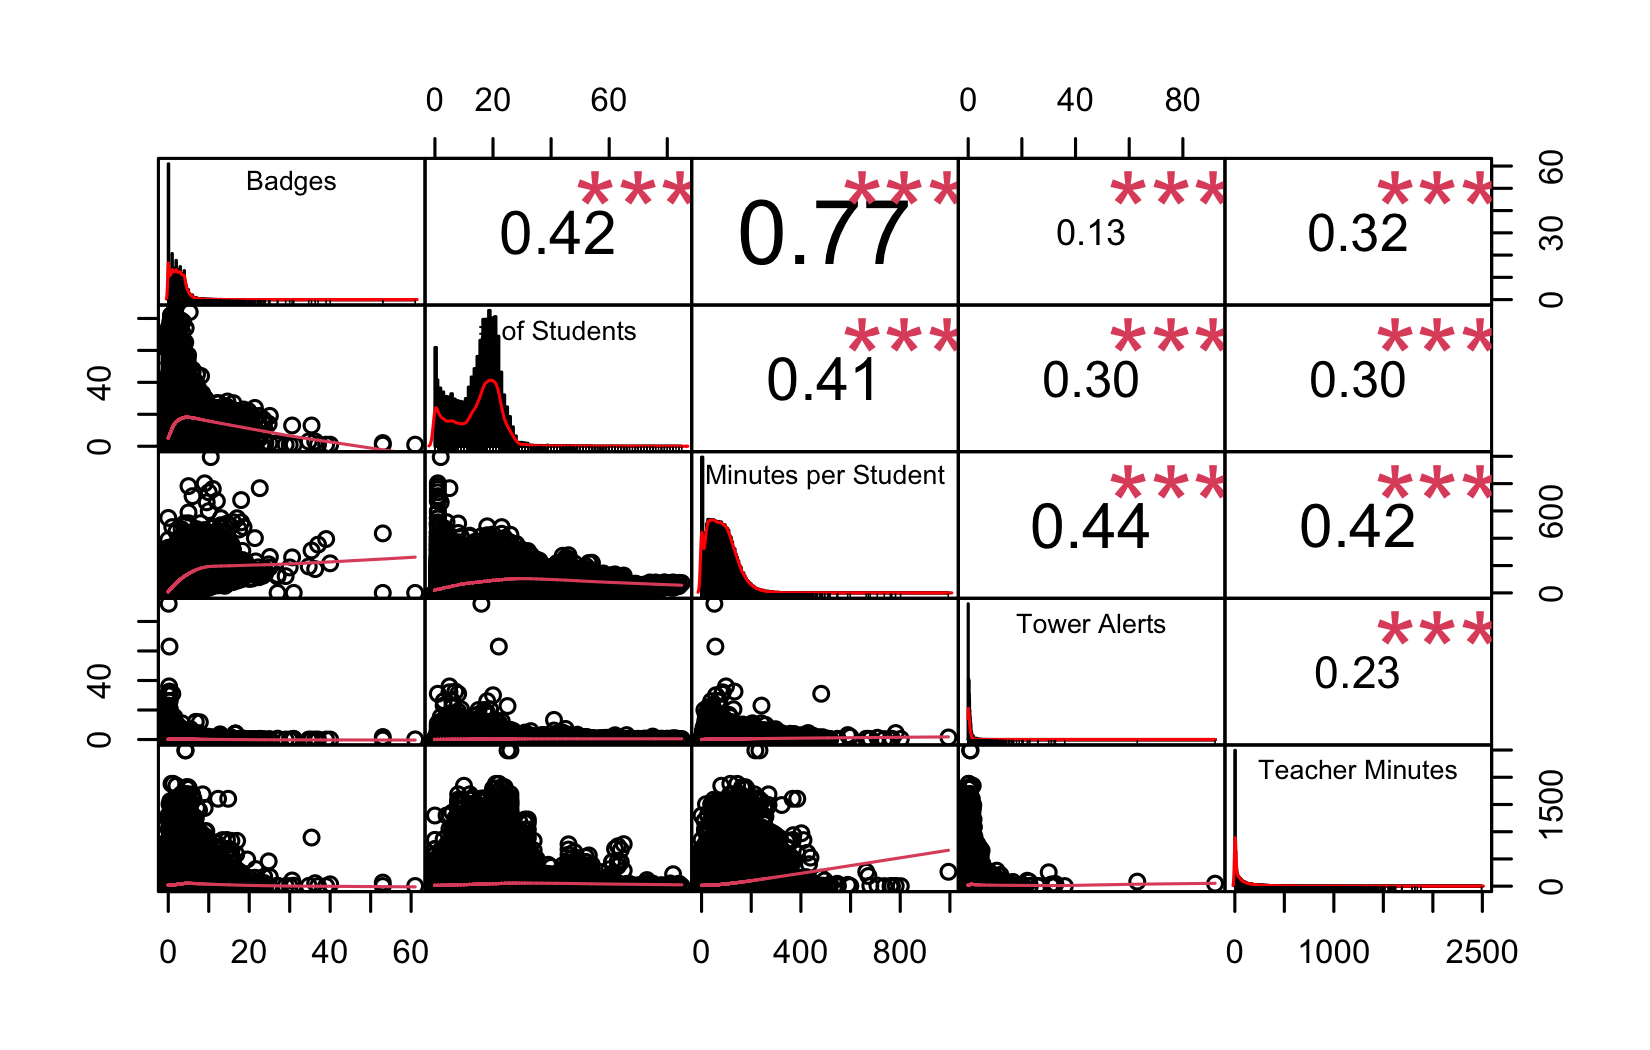
\includegraphics{zearn_files/figure-pdf/fig-corr-1.png}

}

\caption{\label{fig-corr}Correlation coefficients between variables
after stardardization}

\end{figure}%

\subsection{Supplemental Tables}\label{supplemental-tables}

\subsubsection{Teacher Variables}\label{teacher-variables}

\begin{longtable}[]{@{}
  >{\raggedright\arraybackslash}p{(\columnwidth - 2\tabcolsep) * \real{0.2347}}
  >{\raggedright\arraybackslash}p{(\columnwidth - 2\tabcolsep) * \real{0.7653}}@{}}
\caption{Catalog of Teacher Activities. This table presents teachers'
actions, including curriculum engagement, downloads of pedagogical
materials, and completion of various interactive components within the
Zearn educational platform.}\label{tbl-teacher-variables}\tabularnewline
\toprule\noalign{}
\begin{minipage}[b]{\linewidth}\raggedright
\textbf{Variable}
\end{minipage} & \begin{minipage}[b]{\linewidth}\raggedright
\textbf{Description}
\end{minipage} \\
\midrule\noalign{}
\endfirsthead
\toprule\noalign{}
\begin{minipage}[b]{\linewidth}\raggedright
\textbf{Variable}
\end{minipage} & \begin{minipage}[b]{\linewidth}\raggedright
\textbf{Description}
\end{minipage} \\
\midrule\noalign{}
\endhead
\bottomrule\noalign{}
\endlastfoot
PD Course Guide Download \citep{zearn2023, zearn2024c} & Detailed agenda
for Professional Development (PD) courses focusing on classroom
implementation, leadership, supporting diverse learners, using data to
inform teaching practices, and accelerating student learning. \\
PD Course Notes Download \citep{zearn2023, zearn2024c} & Professional
development session notes offering insights into effectively using
Zearn's curriculum. \\
Curriculum Map Download \citep{zearn2024d} & Detailed outline of
learning objectives and content. Presents a sequence of interconnected
math concepts across grades, aligning with states' instructional
requirements. \\
Assessments Download \citep{zearn2024e} & Assessments to evaluate
student understanding of the material, including ongoing formative
assessments, digital daily checks, and paper-based unit assessments. \\
Assessments Answer Key Download \citep{zearn2024f} & Solutions for
assessments to aid in grading and feedback. Provides detailed rubrics
for mission-level assessments. \\
Elementary Schedule Download \citep{zearn2024g} & A recommended schedule
for elementary school-level Zearn curriculum activities to guide daily
and weekly instructional planning, ensuring comprehensive coverage of
curriculum content. \\
Grade Level Overview Download \citep{zearn2024h} & Provides a summary of
learning objectives, pacing guidance, key grade-level terminology, a
list of required materials, and details on the standards covered by each
lesson. \\
Kindergarten Schedule Download \citep{zearn2024i} & Recommended
schedules for Kindergarten, supporting structured instruction
planning. \\
Kindergarten Mission Download \citep{zearn2024j} & Details interactive
activities focused on kindergarten-level concepts and their learning
objectives. \\
Mission Overview Download \citep{zearn2024h} & Outlines a mission's
(i.e., learning module) flow of topics, lessons, and assessments;
highlights foundational concepts introduced earlier; lists recently
introduced terms and required materials for teacher-led instruction. \\
Optional Homework Download \citep{zearn2024k} & Assignments for
additional practice, enhancing student learning outside of class. \\
Optional Problem Sets Download \citep{zearn2024l} & Exercises for extra
practice, tailored to reinforce lesson concepts. \\
Small Group Lesson Download \citep{zearn2024m} & Lessons designed for
small-group engagement. \\
Student Notes and Exit Tickets Download {[}\citep{zearn2024n};
@zearn2024o{]} & Student notes supplement digital lessons with
paper-and-pencil activities. Exit tickets are lesson-level assessments
for teachers to monitor daily learning. \\
Teaching and Learning Approach Download \citep{zearn2024p} & Resources
outlining Zearn's pedagogical methods. \\
Whole Group Fluency Download \citep{zearn2024q} & Lesson-aligned
practice activities to build math fluency through whole-class
engagement. \\
Whole Group Word Problems Download \citep{zearn2024m} & Word
problem-solving activities intended for collaborative, whole-class
engagement. \\
Fluency Completed \citep{zearn2024q} & Indicates teacher completed a
fluency activity, typically given to students before their daily digital
lessons. \\
Guided Practice Completed \citep{zearn2024r} & Indicates teacher
completed a guided practice segment, where students learn new concepts.
These include videos with on-screen teachers, interactive activities,
and paper-and-pencil Student Notes. \\
Kindergarten Activity Completed \citep{zearn2024s} & Indicates teacher
completed an activity within the Kindergarten curriculum. \\
Number Gym Activity Completed \citep{zearn2024t} & Indicates teacher
completed a Number Gym, an individually adaptive activity that builds
number sense, reinforces previously learned skills, and addresses areas
of unfinished learning. \\
Tower Completed \citep{zearn2024b} & Indicates teacher completed a Tower
of Power, an activity that requires full mastery of lesson objectives
and that students must complete independently. \\
Tower Struggled \citep{zearn2024u} & Indicates teacher committed a
mistake when engaging with the Tower of Power activity in a student
role, triggering a ``boost'' (scaffolding remediation). \\
Tower Stage Failed \citep{zearn2024b} & Indicates teacher received three
consecutive ``boosts'' due to repeated errors when engaging with the
Tower of Power in a student role. \\
\end{longtable}

\newpage{}

\begin{table}

\caption{\label{tbl-heterogeneity-reg}Relationship between Q-learning
Model Parameters and Classroom Characteristics. The table presents the
results of five regression models examining how reinforcement learning
(RL) parameters predict income and poverty levels, number of students,
number of classes per teacher, and whether the school had a paid Zearn
subscription. Coefficients and standard errors (in parentheses) are
provided for each parameter. Income and Poverty are treated as ordinal
variables, while Total Students and Number of Classes are count
variables. Paid Account is a binary variable. All RL parameters are
standardized (z-scored) before analysis.}

\centering{

\begin{verbatim}

% Table created by stargazer v.5.2.3 by Marek Hlavac, Social Policy Institute. E-mail: marek.hlavac at gmail.com
% Date and time: Tue, Sep 24, 2024 - 10:52:30
% Requires LaTeX packages: dcolumn 
\begin{table}[!htbp] \centering 
  \caption{Relationship between RL Parameters and Classroom Characteristics} 
  \label{} 
\begin{tabular}{@{\extracolsep{5pt}}lD{.}{.}{-3} D{.}{.}{-3} D{.}{.}{-3} D{.}{.}{-3} D{.}{.}{-3} } 
\\[-1.8ex]\hline 
\hline \\[-1.8ex] 
 & \multicolumn{5}{c}{\textit{Dependent variable:}} \\ 
\cline{2-6} 
\\[-1.8ex] & \multicolumn{1}{c}{Income} & \multicolumn{1}{c}{Poverty} & \multicolumn{1}{c}{Total Students} & \multicolumn{1}{c}{No. of Classes} & \multicolumn{1}{c}{Paid Account} \\ 
\\[-1.8ex] & \multicolumn{1}{c}{\textit{ordered}} & \multicolumn{1}{c}{\textit{ordered}} & \multicolumn{1}{c}{\textit{Poisson}} & \multicolumn{1}{c}{\textit{Poisson}} & \multicolumn{1}{c}{\textit{logistic}} \\ 
 & \multicolumn{1}{c}{\textit{logistic}} & \multicolumn{1}{c}{\textit{logistic}} & \multicolumn{1}{c}{\textit{}} & \multicolumn{1}{c}{\textit{}} & \multicolumn{1}{c}{\textit{}} \\ 
\\[-1.8ex] & \multicolumn{1}{c}{(1)} & \multicolumn{1}{c}{(2)} & \multicolumn{1}{c}{(3)} & \multicolumn{1}{c}{(4)} & \multicolumn{1}{c}{(5)}\\ 
\hline \\[-1.8ex] 
 Learning Rate ($\alpha$) & -0.119^{*} & 0.032 & 0.006 & 0.021 & 0.208^{*} \\ 
  & (0.049) & (0.056) & (0.006) & (0.019) & (0.084) \\ 
  & & & & & \\ 
 Discount Factor ($\gamma$) & 0.021 & 0.112 & -0.006 & -0.038 & 0.003 \\ 
  & (0.057) & (0.064) & (0.007) & (0.022) & (0.104) \\ 
  & & & & & \\ 
 Inverse Temperature ($\tau$) & -0.018 & -0.066 & 0.007 & -0.023 & 0.093 \\ 
  & (0.050) & (0.053) & (0.006) & (0.021) & (0.080) \\ 
  & & & & & \\ 
 Initial Q-value & 0.232^{***} & 0.086 & 0.001 & -0.007 & -0.239^{*} \\ 
  & (0.056) & (0.063) & (0.007) & (0.021) & (0.099) \\ 
  & & & & & \\ 
 Cost & -0.260^{***} & 0.218^{***} & -0.014^{*} & -0.059^{**} & 0.609^{***} \\ 
  & (0.052) & (0.061) & (0.006) & (0.020) & (0.122) \\ 
  & & & & & \\ 
 Constant &  &  & 3.027^{***} & 0.756^{***} & 2.139^{***} \\ 
  &  &  & (0.005) & (0.016) & (0.086) \\ 
  & & & & & \\ 
\hline \\[-1.8ex] 
Observations & \multicolumn{1}{c}{1,737} & \multicolumn{1}{c}{1,668} & \multicolumn{1}{c}{1,782} & \multicolumn{1}{c}{1,782} & \multicolumn{1}{c}{1,782} \\ 
Log Likelihood &  &  & \multicolumn{1}{c}{-5,728.112} & \multicolumn{1}{c}{-2,671.142} & \multicolumn{1}{c}{-628.732} \\ 
Akaike Inf. Crit. &  &  & \multicolumn{1}{c}{11,468.220} & \multicolumn{1}{c}{5,354.284} & \multicolumn{1}{c}{1,269.464} \\ 
\hline 
\hline \\[-1.8ex] 
\textit{Note:}  & \multicolumn{5}{r}{$^{*}$p$<$0.05; $^{**}$p$<$0.01; $^{***}$p$<$0.001} \\ 
\end{tabular} 
\end{table} 
\end{verbatim}

}

\end{table}%

\begin{table}

\caption{\label{tbl-optimality-2}Impact of Q-learning Model Parameters
on Average Weekly Tower Alerts per Tower Completion. Three linear
regression models examine the correlations between a teacher's
reinforcement learning (RL) parameters and student struggle, measured by
average weekly Tower Alerts. Model 1 includes only RL parameters. Model
2 adds controls for AIC, number of weeks, total students, and number of
classes. Model 3 further incorporates controls for grade level, poverty
level, charter school status, and whether the school has a paid Zearn
account. Coefficients and standard errors (in parentheses) are provided
for each parameter.}

\centering{

[!htbp] \centering 
  \caption{} 
  \label{} 
\begin{tabular}{@{\extracolsep{5pt}}lD{.}{.}{-3} D{.}{.}{-3} D{.}{.}{-3} } 
\\[-1.8ex]\hline 
\hline \\[-1.8ex] 
 & \multicolumn{3}{c}{\textit{Dependent variable:}} \\ 
\cline{2-4} 
\\[-1.8ex] & \multicolumn{3}{c}{Tower Alerts} \\ 
\\[-1.8ex] & \multicolumn{1}{c}{(1)} & \multicolumn{1}{c}{(2)} & \multicolumn{1}{c}{(3)}\\ 
\hline \\[-1.8ex] 
 $\alpha$ & 0.061^{***} & 0.059^{***} & 0.050^{***} \\ 
  & (0.015) & (0.015) & (0.015) \\ 
  & & & \\ 
 $\gamma$ & 0.006 & 0.015 & 0.023 \\ 
  & (0.017) & (0.017) & (0.017) \\ 
  & & & \\ 
 $\tau$ & -0.019 & -0.023 & -0.023 \\ 
  & (0.015) & (0.016) & (0.015) \\ 
  & & & \\ 
 Cost & 0.031^{*} & 0.031 & 0.042^{*} \\ 
  & (0.016) & (0.021) & (0.021) \\ 
  & & & \\ 
 Starting Q-value & -0.019 & -0.013 & -0.002 \\ 
  & (0.017) & (0.019) & (0.018) \\ 
  & & & \\ 
 No. of Weeks &  & 0.008^{**} & 0.007^{**} \\ 
  &  & (0.003) & (0.003) \\ 
  & & & \\ 
 No. of Students &  & -0.006^{**} & -0.008^{***} \\ 
  &  & (0.002) & (0.002) \\ 
  & & & \\ 
 No. of Classes &  & 0.066^{***} & -0.007 \\ 
  &  & (0.013) & (0.016) \\ 
  & & & \\ 
 Charter School &  &  & -0.026 \\ 
  &  &  & (0.052) \\ 
  & & & \\ 
 Paid Zearn Account &  &  & 0.130^{***} \\ 
  &  &  & (0.038) \\ 
  & & & \\ 
 Constant & 0.934^{***} & 0.730^{***} & -0.157 \\ 
  & (0.013) & (0.080) & (0.172) \\ 
  & & & \\ 
\hline \\[-1.8ex] 
Control for AIC &  & Yes & Yes \\ 
Control for Grade Level &  &  & Yes \\ 
Control for Poverty Level &  &  & Yes \\ 
Observations & \multicolumn{1}{c}{1,782} & \multicolumn{1}{c}{1,782} & \multicolumn{1}{c}{1,668} \\ 
R$^{2}$ & \multicolumn{1}{c}{0.026} & \multicolumn{1}{c}{0.051} & \multicolumn{1}{c}{0.162} \\ 
Adjusted R$^{2}$ & \multicolumn{1}{c}{0.023} & \multicolumn{1}{c}{0.046} & \multicolumn{1}{c}{0.153} \\ 
Residual Std. Error & \multicolumn{1}{c}{0.534 (df = 1776)} & \multicolumn{1}{c}{0.527 (df = 1772)} & \multicolumn{1}{c}{0.498 (df = 1649)} \\ 
F Statistic & \multicolumn{1}{c}{9.479$^{***}$ (df = 5; 1776)} & \multicolumn{1}{c}{10.646$^{***}$ (df = 9; 1772)} & \multicolumn{1}{c}{17.683$^{***}$ (df = 18; 1649)} \\ 
\hline 
\hline \\[-1.8ex] 
\textit{Note:}  & \multicolumn{3}{r}{$^{*}$p$<$0.05; $^{**}$p$<$0.01; $^{***}$p$<$0.001} \\ 
\end{tabular} 

}

\end{table}%

\subsection{Supplemental Figures}\label{sec-supp-fig}

\begin{figure}

\centering{

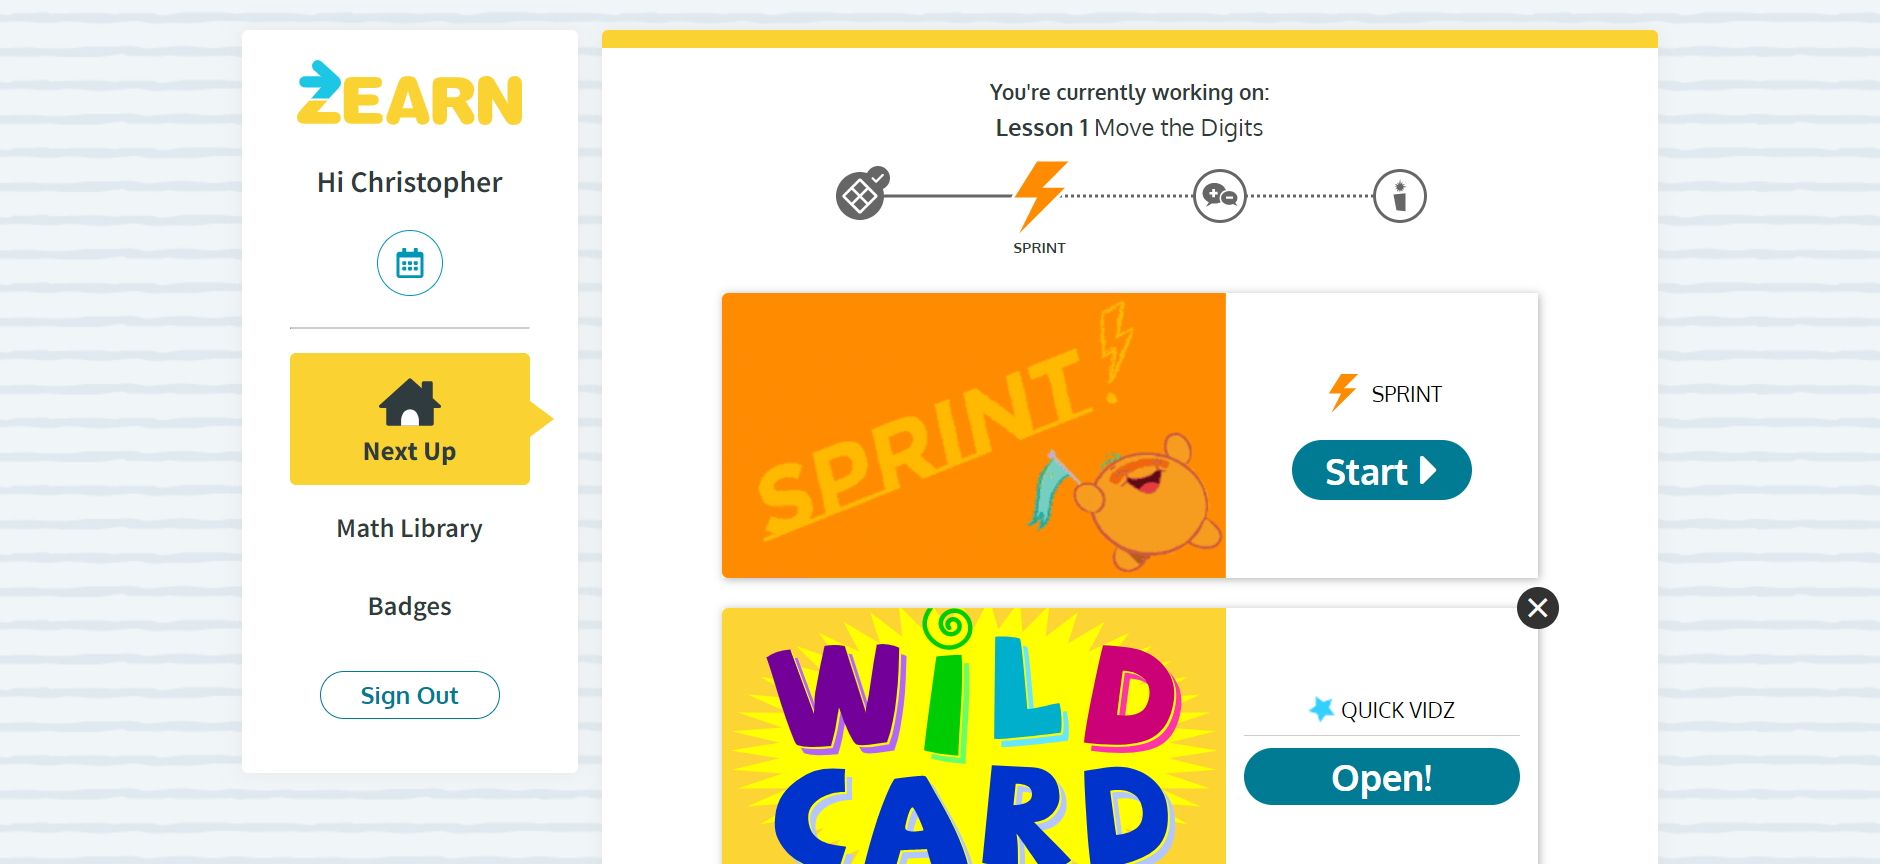
\includegraphics{images/student-feed.PNG}

}

\caption{\label{fig-st-portal}Zearn Student Portal}

\end{figure}%

\begin{figure}

\centering{

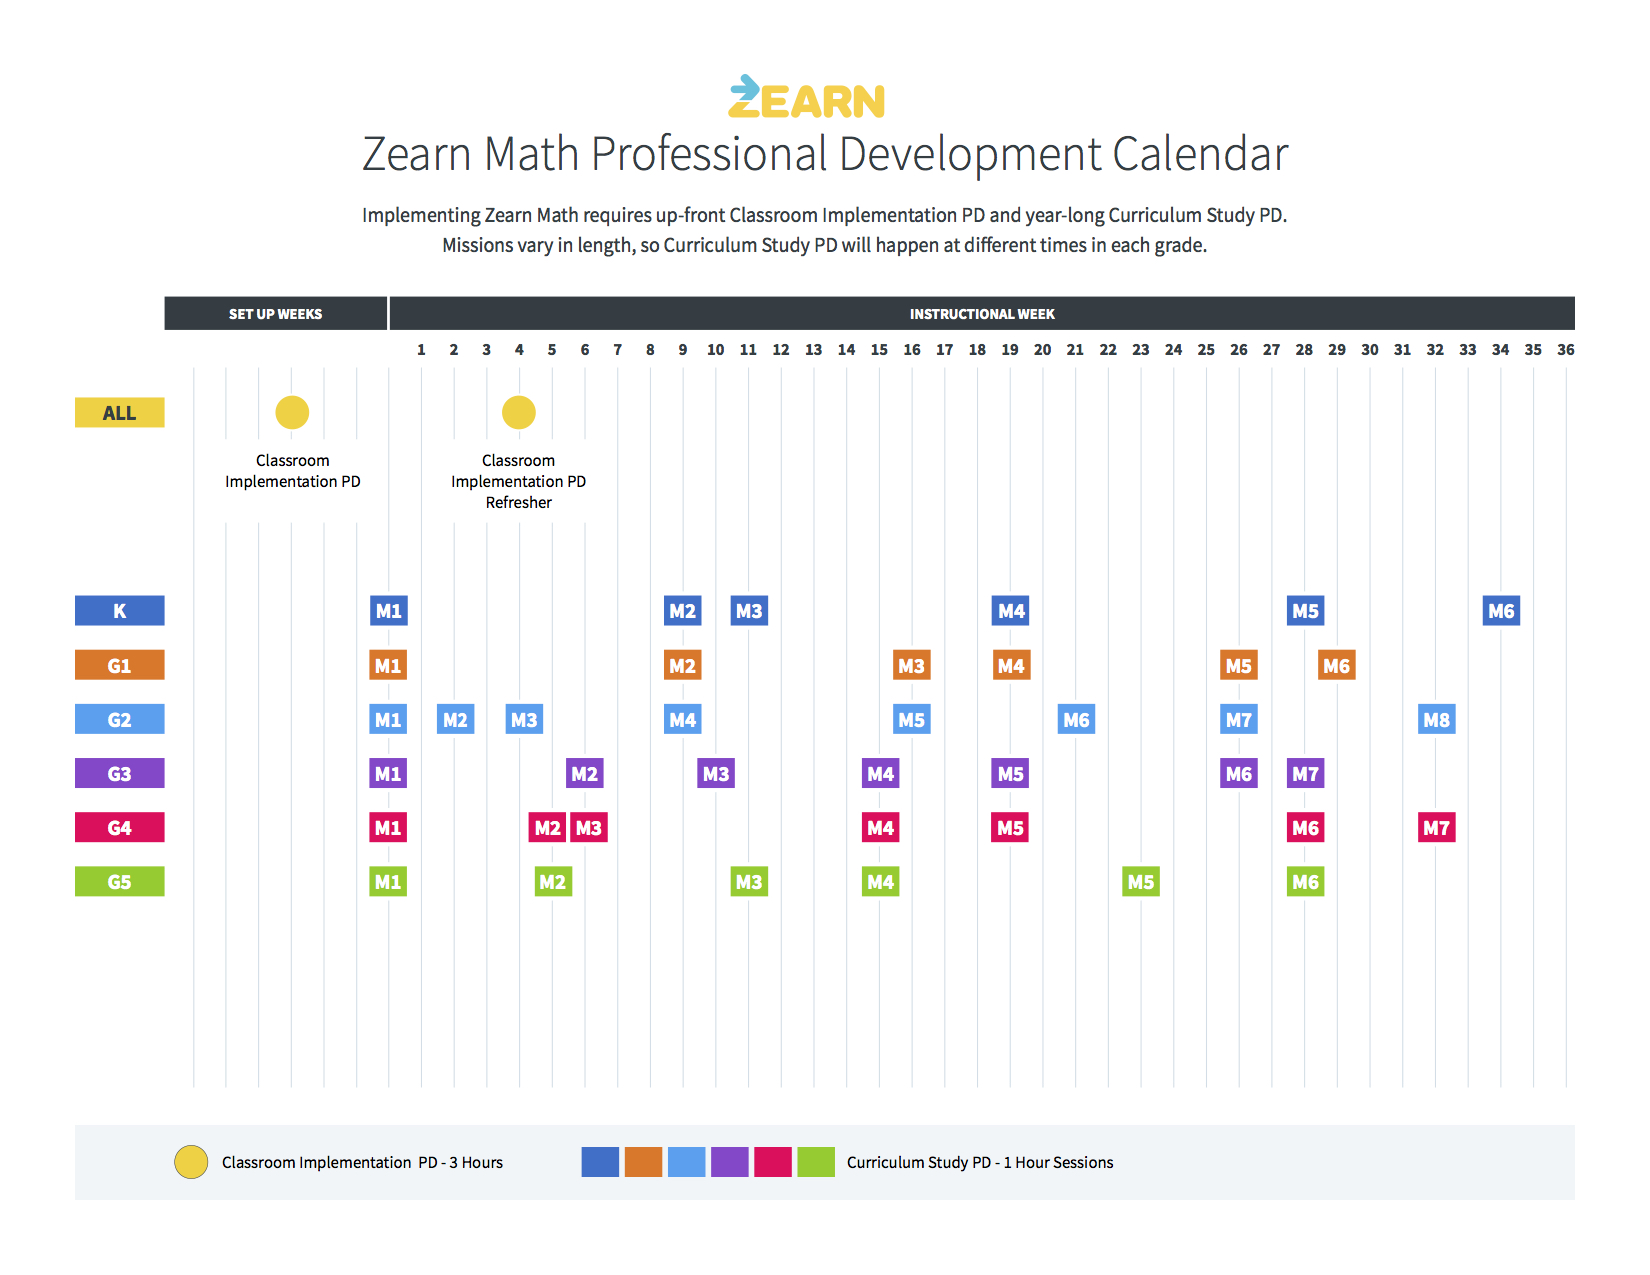
\includegraphics{images/PD-calendar.jpg}

}

\caption{\label{fig-prof-dev}Professional Development Calendar}

\end{figure}%

\newpage{}

\begin{figure}

\begin{minipage}{0.50\linewidth}

\centering{

\includegraphics{zearn_files/figure-pdf/fig-income-dist-1.pdf}

}

\subcaption{\label{fig-income-dist-1}School Poverty Distribution}

\end{minipage}%
%
\begin{minipage}{0.50\linewidth}

\centering{

\includegraphics{zearn_files/figure-pdf/fig-income-dist-2.pdf}

}

\subcaption{\label{fig-income-dist-2}Median Income Distribution}

\end{minipage}%

\caption{\label{fig-income-dist}Distributions of School Socioeconomic
Profiles. The first graph categorizes schools into three groups based on
the percentage of students eligible for free or reduced-price lunch
(FRPL): low-poverty (0-40\%), mid-poverty (40-75\%), and high-poverty
(over 75\%). The second graph presents the distribution of median
incomes for a school's associated region.}

\end{figure}%

\begin{figure}

\centering{

\includegraphics{zearn_files/figure-pdf/fig-teachers-map-1.pdf}

}

\caption{\label{fig-teachers-map}Geographic distribution of Zearn
teachers across parishes in Louisiana. The color gradient represents the
density of teachers, with darker hues indicating a higher concentration
of educators using Zearn in each parish. The map also labels the top
five cities where Zearn adoption is most prevalent.}

\end{figure}%

\begin{figure}

\centering{

\includegraphics{zearn_files/figure-pdf/fig-logins-week-1.pdf}

}

\caption{\label{fig-logins-week}Total number of student logins over the
2019-2020 school year. The chart depicts the connection between academic
schedules and platform engagement. Each bar represents a week, with
peaks corresponding to active school weeks and troughs aligning with
major holiday periods (e.g., Thanksgiving and Winter Break).}

\end{figure}%

\begin{figure}

\centering{

\includegraphics{zearn_files/figure-pdf/fig-loglik-histogram-1.pdf}

}

\caption{\label{fig-loglik-histogram}Distribution of teacher-specific
Bayesian Information Criteria (BIC). The histogram displays the spread
of individual teachers' log-likelihoods, with higher values indicating
better fit. The dashed line represents the median log-likelihood across
all teachers.}

\end{figure}%





\end{document}
